% Generated by Sphinx.
\def\sphinxdocclass{report}
\documentclass[letterpaper,10pt,english]{sphinxmanual}
\usepackage[utf8]{inputenc}
\DeclareUnicodeCharacter{00A0}{\nobreakspace}
\usepackage[T1]{fontenc}
\usepackage{babel}
\usepackage{times}
\usepackage[Bjarne]{fncychap}
\usepackage{longtable}
\usepackage{sphinx}
\usepackage{multirow}


\title{Authentic2 Documentation}
\date{October 20, 2011}
\release{1.9.2}
\author{Mikaël Ates}
\newcommand{\sphinxlogo}{}
\renewcommand{\releasename}{Release}
\makeindex

\makeatletter
\def\PYG@reset{\let\PYG@it=\relax \let\PYG@bf=\relax%
    \let\PYG@ul=\relax \let\PYG@tc=\relax%
    \let\PYG@bc=\relax \let\PYG@ff=\relax}
\def\PYG@tok#1{\csname PYG@tok@#1\endcsname}
\def\PYG@toks#1+{\ifx\relax#1\empty\else%
    \PYG@tok{#1}\expandafter\PYG@toks\fi}
\def\PYG@do#1{\PYG@bc{\PYG@tc{\PYG@ul{%
    \PYG@it{\PYG@bf{\PYG@ff{#1}}}}}}}
\def\PYG#1#2{\PYG@reset\PYG@toks#1+\relax+\PYG@do{#2}}

\def\PYG@tok@gd{\def\PYG@tc##1{\textcolor[rgb]{0.63,0.00,0.00}{##1}}}
\def\PYG@tok@gu{\let\PYG@bf=\textbf\def\PYG@tc##1{\textcolor[rgb]{0.50,0.00,0.50}{##1}}}
\def\PYG@tok@gt{\def\PYG@tc##1{\textcolor[rgb]{0.00,0.25,0.82}{##1}}}
\def\PYG@tok@gs{\let\PYG@bf=\textbf}
\def\PYG@tok@gr{\def\PYG@tc##1{\textcolor[rgb]{1.00,0.00,0.00}{##1}}}
\def\PYG@tok@cm{\let\PYG@it=\textit\def\PYG@tc##1{\textcolor[rgb]{0.25,0.50,0.56}{##1}}}
\def\PYG@tok@vg{\def\PYG@tc##1{\textcolor[rgb]{0.73,0.38,0.84}{##1}}}
\def\PYG@tok@m{\def\PYG@tc##1{\textcolor[rgb]{0.13,0.50,0.31}{##1}}}
\def\PYG@tok@mh{\def\PYG@tc##1{\textcolor[rgb]{0.13,0.50,0.31}{##1}}}
\def\PYG@tok@cs{\def\PYG@tc##1{\textcolor[rgb]{0.25,0.50,0.56}{##1}}\def\PYG@bc##1{\colorbox[rgb]{1.00,0.94,0.94}{##1}}}
\def\PYG@tok@ge{\let\PYG@it=\textit}
\def\PYG@tok@vc{\def\PYG@tc##1{\textcolor[rgb]{0.73,0.38,0.84}{##1}}}
\def\PYG@tok@il{\def\PYG@tc##1{\textcolor[rgb]{0.13,0.50,0.31}{##1}}}
\def\PYG@tok@go{\def\PYG@tc##1{\textcolor[rgb]{0.19,0.19,0.19}{##1}}}
\def\PYG@tok@cp{\def\PYG@tc##1{\textcolor[rgb]{0.00,0.44,0.13}{##1}}}
\def\PYG@tok@gi{\def\PYG@tc##1{\textcolor[rgb]{0.00,0.63,0.00}{##1}}}
\def\PYG@tok@gh{\let\PYG@bf=\textbf\def\PYG@tc##1{\textcolor[rgb]{0.00,0.00,0.50}{##1}}}
\def\PYG@tok@ni{\let\PYG@bf=\textbf\def\PYG@tc##1{\textcolor[rgb]{0.84,0.33,0.22}{##1}}}
\def\PYG@tok@nl{\let\PYG@bf=\textbf\def\PYG@tc##1{\textcolor[rgb]{0.00,0.13,0.44}{##1}}}
\def\PYG@tok@nn{\let\PYG@bf=\textbf\def\PYG@tc##1{\textcolor[rgb]{0.05,0.52,0.71}{##1}}}
\def\PYG@tok@no{\def\PYG@tc##1{\textcolor[rgb]{0.38,0.68,0.84}{##1}}}
\def\PYG@tok@na{\def\PYG@tc##1{\textcolor[rgb]{0.25,0.44,0.63}{##1}}}
\def\PYG@tok@nb{\def\PYG@tc##1{\textcolor[rgb]{0.00,0.44,0.13}{##1}}}
\def\PYG@tok@nc{\let\PYG@bf=\textbf\def\PYG@tc##1{\textcolor[rgb]{0.05,0.52,0.71}{##1}}}
\def\PYG@tok@nd{\let\PYG@bf=\textbf\def\PYG@tc##1{\textcolor[rgb]{0.33,0.33,0.33}{##1}}}
\def\PYG@tok@ne{\def\PYG@tc##1{\textcolor[rgb]{0.00,0.44,0.13}{##1}}}
\def\PYG@tok@nf{\def\PYG@tc##1{\textcolor[rgb]{0.02,0.16,0.49}{##1}}}
\def\PYG@tok@si{\let\PYG@it=\textit\def\PYG@tc##1{\textcolor[rgb]{0.44,0.63,0.82}{##1}}}
\def\PYG@tok@s2{\def\PYG@tc##1{\textcolor[rgb]{0.25,0.44,0.63}{##1}}}
\def\PYG@tok@vi{\def\PYG@tc##1{\textcolor[rgb]{0.73,0.38,0.84}{##1}}}
\def\PYG@tok@nt{\let\PYG@bf=\textbf\def\PYG@tc##1{\textcolor[rgb]{0.02,0.16,0.45}{##1}}}
\def\PYG@tok@nv{\def\PYG@tc##1{\textcolor[rgb]{0.73,0.38,0.84}{##1}}}
\def\PYG@tok@s1{\def\PYG@tc##1{\textcolor[rgb]{0.25,0.44,0.63}{##1}}}
\def\PYG@tok@gp{\let\PYG@bf=\textbf\def\PYG@tc##1{\textcolor[rgb]{0.78,0.36,0.04}{##1}}}
\def\PYG@tok@sh{\def\PYG@tc##1{\textcolor[rgb]{0.25,0.44,0.63}{##1}}}
\def\PYG@tok@ow{\let\PYG@bf=\textbf\def\PYG@tc##1{\textcolor[rgb]{0.00,0.44,0.13}{##1}}}
\def\PYG@tok@sx{\def\PYG@tc##1{\textcolor[rgb]{0.78,0.36,0.04}{##1}}}
\def\PYG@tok@bp{\def\PYG@tc##1{\textcolor[rgb]{0.00,0.44,0.13}{##1}}}
\def\PYG@tok@c1{\let\PYG@it=\textit\def\PYG@tc##1{\textcolor[rgb]{0.25,0.50,0.56}{##1}}}
\def\PYG@tok@kc{\let\PYG@bf=\textbf\def\PYG@tc##1{\textcolor[rgb]{0.00,0.44,0.13}{##1}}}
\def\PYG@tok@c{\let\PYG@it=\textit\def\PYG@tc##1{\textcolor[rgb]{0.25,0.50,0.56}{##1}}}
\def\PYG@tok@mf{\def\PYG@tc##1{\textcolor[rgb]{0.13,0.50,0.31}{##1}}}
\def\PYG@tok@err{\def\PYG@bc##1{\fcolorbox[rgb]{1.00,0.00,0.00}{1,1,1}{##1}}}
\def\PYG@tok@kd{\let\PYG@bf=\textbf\def\PYG@tc##1{\textcolor[rgb]{0.00,0.44,0.13}{##1}}}
\def\PYG@tok@ss{\def\PYG@tc##1{\textcolor[rgb]{0.32,0.47,0.09}{##1}}}
\def\PYG@tok@sr{\def\PYG@tc##1{\textcolor[rgb]{0.14,0.33,0.53}{##1}}}
\def\PYG@tok@mo{\def\PYG@tc##1{\textcolor[rgb]{0.13,0.50,0.31}{##1}}}
\def\PYG@tok@mi{\def\PYG@tc##1{\textcolor[rgb]{0.13,0.50,0.31}{##1}}}
\def\PYG@tok@kn{\let\PYG@bf=\textbf\def\PYG@tc##1{\textcolor[rgb]{0.00,0.44,0.13}{##1}}}
\def\PYG@tok@o{\def\PYG@tc##1{\textcolor[rgb]{0.40,0.40,0.40}{##1}}}
\def\PYG@tok@kr{\let\PYG@bf=\textbf\def\PYG@tc##1{\textcolor[rgb]{0.00,0.44,0.13}{##1}}}
\def\PYG@tok@s{\def\PYG@tc##1{\textcolor[rgb]{0.25,0.44,0.63}{##1}}}
\def\PYG@tok@kp{\def\PYG@tc##1{\textcolor[rgb]{0.00,0.44,0.13}{##1}}}
\def\PYG@tok@w{\def\PYG@tc##1{\textcolor[rgb]{0.73,0.73,0.73}{##1}}}
\def\PYG@tok@kt{\def\PYG@tc##1{\textcolor[rgb]{0.56,0.13,0.00}{##1}}}
\def\PYG@tok@sc{\def\PYG@tc##1{\textcolor[rgb]{0.25,0.44,0.63}{##1}}}
\def\PYG@tok@sb{\def\PYG@tc##1{\textcolor[rgb]{0.25,0.44,0.63}{##1}}}
\def\PYG@tok@k{\let\PYG@bf=\textbf\def\PYG@tc##1{\textcolor[rgb]{0.00,0.44,0.13}{##1}}}
\def\PYG@tok@se{\let\PYG@bf=\textbf\def\PYG@tc##1{\textcolor[rgb]{0.25,0.44,0.63}{##1}}}
\def\PYG@tok@sd{\let\PYG@it=\textit\def\PYG@tc##1{\textcolor[rgb]{0.25,0.44,0.63}{##1}}}

\def\PYGZbs{\char`\\}
\def\PYGZus{\char`\_}
\def\PYGZob{\char`\{}
\def\PYGZcb{\char`\}}
\def\PYGZca{\char`\^}
\def\PYGZsh{\char`\#}
\def\PYGZpc{\char`\%}
\def\PYGZdl{\char`\$}
\def\PYGZti{\char`\~}
% for compatibility with earlier versions
\def\PYGZat{@}
\def\PYGZlb{[}
\def\PYGZrb{]}
\makeatother

\begin{document}

\maketitle
\tableofcontents
\phantomsection\label{index::doc}


Authentic2 is a versatile identity provider addressing a broad
range of needs, from simple to advanced setups, around web authentication,
attribute sharing, namespace mapping and authorization management.

Authentic2 supports many protocols and standards, including SAML2, CAS, OpenID,
LDAP, X509, OATH, and can bridge between them.

Authentic2 is under the GNU AGPL version 3 licence.

It has support for SAMLv2 thanks to \href{http://lasso.entrouvert.org}{Lasso},
a free (GNU GPL) implementation of the Liberty Alliance and OASIS
specifications of SAML2, ID-FF1.2 and ID-WSF2.
\begin{itemize}
\item {} 
\href{http://dev.entrouvert.org/projects/authentic}{Authentic2 project site}

\item {} 
\href{http://dev.entrouvert.org/projects/authentic/roadmap}{Authentic2 roadmap}

\end{itemize}


\chapter{Documentation content}
\label{index:authentic2-s-documentation}\label{index:documentation-content}

\section{Features}
\label{features::doc}\label{features:features}\label{features:id1}
Authentic can authenticate users against:
\begin{itemize}
\item {} 
an LDAP directory,

\item {} 
a SAML 2.0 identity provider,

\item {} 
an OpenID identity provider,

\item {} 
with an X509 certificate.

\end{itemize}

Authentic can provide authentication to web applications using the following
protocols:
\begin{itemize}
\item {} 
OpenID,

\item {} 
SAML 2.0,

\item {} 
CAS 1.0 \& CAS 2.0.

\end{itemize}

Authentic can proxy authentication between any two different protocols it
support.


\section{Download}
\label{download:download}\label{download::doc}\label{download:id1}\begin{enumerate}
\item {} 
Pypi: \href{http://pypi.python.org/pypi/authentic2/1.9.0}{http://pypi.python.org/pypi/authentic2/1.9.0}

\item {} 
Git repository: \href{http://repos.entrouvert.org/authentic.git}{http://repos.entrouvert.org/authentic.git}

\item {} 
\href{http://dev.entrouvert.org/projects/authentic/repository}{Browse source}

\end{enumerate}


\section{Installation}
\label{installation:installation}\label{installation::doc}\label{installation:id1}

\subsection{Dependencies}
\label{installation:dependencies}
You must install the following packages to use Authentic
\begin{itemize}
\item {} 
Python Lasso binding 2.3.5:
\begin{quote}

From sources: \href{http://lasso.entrouvert.org/download}{http://lasso.entrouvert.org/download}
Debian based distribution: apt-get install python-lasso
\end{quote}

\item {} 
Django 1.3:
\begin{quote}

From sources: \href{http://www.djangoproject.com/download/1.3/tarball/}{http://www.djangoproject.com/download/1.3/tarball/}
\end{quote}

\item {} 
Django-registration 0.8-alpha-1:
\begin{quote}

From sources: \href{http://bitbucket.org/ubernostrum/django-registration/downloads}{http://bitbucket.org/ubernostrum/django-registration/downloads}
Debian based distribution: apt-get install python-django-registration
\end{quote}

\item {} 
Django-authopenid 0.9.6:
\begin{quote}

From sources: \href{http://bitbucket.org/benoitc/django-authopenid/downloads}{http://bitbucket.org/benoitc/django-authopenid/downloads}
\end{quote}

\item {} 
Django-south 0.7.3:
\begin{quote}

From sources:: \href{http://south.aeracode.org/docs/installation.html}{http://south.aeracode.org/docs/installation.html}
\end{quote}

\item {} 
Django-profiles 0.2:
\begin{quote}

From sources:: \href{http://pypi.python.org/pypi/django-profiles}{http://pypi.python.org/pypi/django-profiles}
\end{quote}

\end{itemize}

You install all the django libraries quickly using pip:

\begin{Verbatim}[commandchars=\\\{\}]
pip install django django-profiles django-registration \PYGZbs{}
            django-debug-toolbar django-authopenid south
\end{Verbatim}

or easy\_install:

\begin{Verbatim}[commandchars=\\\{\}]
easy\_install django django-profiles django-registration \PYGZbs{}
             django-debug-toolbar django-authopenid south
\end{Verbatim}


\subsection{Quick Start}
\label{installation:quick-start}
Then launch the following commands:

\begin{Verbatim}[commandchars=\\\{\}]
python manage.py syncdb --migrate
python manage.py runserver
\end{Verbatim}

You should see the following output:

\begin{Verbatim}[commandchars=\\\{\}]
Validating models...
0 errors found

Django version 1.2, using settings 'authentic.settings'
Development server is running at http://127.0.0.1:8000/
Quit the server with CONTROL-C.

You can access the running application on http://127.0.0.1:8000/
\end{Verbatim}


\subsection{Specifying a different database}
\label{installation:specifying-a-different-database}
This is done by modifying the DATABASES dictionary in your local\_settings.py file
(create it in Authentic project directory); for example:

\begin{Verbatim}[commandchars=\\\{\}]
\PYG{n}{DATABASES}\PYG{p}{[}\PYG{l+s}{'}\PYG{l+s}{default}\PYG{l+s}{'}\PYG{p}{]} \PYG{o}{=} \PYG{p}{\PYGZob{}}
  \PYG{l+s}{'}\PYG{l+s}{ENGINE}\PYG{l+s}{'}\PYG{p}{:} \PYG{l+s}{'}\PYG{l+s}{django.db.backends.postgresql}\PYG{l+s}{'}\PYG{p}{,}
  \PYG{l+s}{'}\PYG{l+s}{NAME}\PYG{l+s}{'}\PYG{p}{:} \PYG{l+s}{'}\PYG{l+s}{authentic}\PYG{l+s}{'}\PYG{p}{,}
  \PYG{l+s}{'}\PYG{l+s}{USER}\PYG{l+s}{'}\PYG{p}{:} \PYG{l+s}{'}\PYG{l+s}{admindb}\PYG{l+s}{'}\PYG{p}{,}
  \PYG{l+s}{'}\PYG{l+s}{PASSWORD}\PYG{l+s}{'}\PYG{p}{:} \PYG{l+s}{'}\PYG{l+s}{foobar}\PYG{l+s}{'}\PYG{p}{,}
  \PYG{l+s}{'}\PYG{l+s}{HOST}\PYG{l+s}{'}\PYG{p}{:} \PYG{l+s}{'}\PYG{l+s}{db.example.com}\PYG{l+s}{'}\PYG{p}{,}
  \PYG{l+s}{'}\PYG{l+s}{PORT}\PYG{l+s}{'}\PYG{p}{:} \PYG{l+s}{'}\PYG{l+s}{'}\PYG{p}{,} \PYG{c}{\PYGZsh{} empty string means default value}
\PYG{p}{\PYGZcb{}}
\end{Verbatim}

You should refer to the Django documentation on databases settings at
\href{http://docs.djangoproject.com/en/dev/ref/settings/\#databases}{http://docs.djangoproject.com/en/dev/ref/settings/\#databases} for all
the details.


\subsection{How to upgrade to a new version of authentic ?}
\label{installation:how-to-upgrade-to-a-new-version-of-authentic}
Authentic store all its data in a relational database as specified in its
settings.py or local\_settings.py file. So in order to upgrade to a new version
of authentic you have to update your database schema using the
migration command — you will need to have installed the dependency django-south,
see the beginning of this README file.:

\begin{Verbatim}[commandchars=\\\{\}]
python ./manage.py migrate
\end{Verbatim}

Then you will need to create new tables if there are.:

\begin{Verbatim}[commandchars=\\\{\}]
python ./manage.py syncdb
\end{Verbatim}


\section{Authentication with an existing LDAP directory}
\label{auth_ldap:auth-ldap}\label{auth_ldap:authentication-with-an-existing-ldap-directory}\label{auth_ldap::doc}
Authentic use the module django\_auth\_ldap to synchronize the Django user tables
with an LDAP. For complex use case, we will refer you to the django\_auth\_ldap
documentation, see \href{http://packages.python.org/django-auth-ldap/}{http://packages.python.org/django-auth-ldap/}.


\subsection{How to authenticate users against an LDAP server with anonymous binding ?}
\label{auth_ldap:how-to-authenticate-users-against-an-ldap-server-with-anonymous-binding}\begin{enumerate}
\item {} 
Install the django\_auth\_ldap module for Django:

\begin{Verbatim}[commandchars=\\\{\}]
pip install django\_auth\_ldap
\end{Verbatim}

\item {} 
Configure your local\_settings.py file for authenticating against LDAP.

\end{enumerate}

The next lines must be added:

\begin{Verbatim}[commandchars=\\\{\}]
\PYG{n}{AUTHENTICATION\PYGZus{}BACKENDS} \PYG{o}{+}\PYG{o}{=} \PYG{p}{(} \PYG{l+s}{'}\PYG{l+s}{django\PYGZus{}auth\PYGZus{}ldap.backend.LDAPBackend}\PYG{l+s}{'}\PYG{p}{,} \PYG{p}{)}

\PYG{k+kn}{import} \PYG{n+nn}{ldap}
\PYG{k+kn}{from} \PYG{n+nn}{django\PYGZus{}auth\PYGZus{}ldap.config} \PYG{k+kn}{import} \PYG{n}{LDAPSearch}

\PYG{c}{\PYGZsh{} Here put the LDAP URL of your server}
\PYG{n}{AUTH\PYGZus{}LDAP\PYGZus{}SERVER\PYGZus{}URI} \PYG{o}{=} \PYG{l+s}{'}\PYG{l+s}{ldap://ldap.example.com}\PYG{l+s}{'}
\PYG{c}{\PYGZsh{} Let the bind DN and bind password blank for anonymous binding}
\PYG{n}{AUTH\PYGZus{}LDAP\PYGZus{}BIND\PYGZus{}DN} \PYG{o}{=} \PYG{l+s}{"}\PYG{l+s}{"}
\PYG{n}{AUTH\PYGZus{}LDAP\PYGZus{}BIND\PYGZus{}PASSWORD} \PYG{o}{=} \PYG{l+s}{"}\PYG{l+s}{"}
\PYG{c}{\PYGZsh{} Lookup user under the branch o=base and by mathcing their uid against the}
\PYG{c}{\PYGZsh{} received login name}
\PYG{n}{AUTH\PYGZus{}LDAP\PYGZus{}USER\PYGZus{}SEARCH} \PYG{o}{=} \PYG{n}{LDAPSearch}\PYG{p}{(}\PYG{l+s}{"}\PYG{l+s}{o=base}\PYG{l+s}{"}\PYG{p}{,}
    \PYG{n}{ldap}\PYG{o}{.}\PYG{n}{SCOPE\PYGZus{}SUBTREE}\PYG{p}{,} \PYG{l+s}{"}\PYG{l+s}{(uid=}\PYG{l+s+si}{\PYGZpc{}(user)s}\PYG{l+s}{)}\PYG{l+s}{"}\PYG{p}{)}
\end{Verbatim}


\subsection{How to allow members of an LDAP group to manage Authentic ?}
\label{auth_ldap:how-to-allow-members-of-an-ldap-group-to-manage-authentic}\begin{enumerate}
\item {} 
First you must know the objectClass of groups in your LDAP schema, this FAQ
will show you the configuration for two usual classes: groupOfNames and
groupOfUniqueNames.

\item {} 
Find the relevant groupname. We will say it is: cn=admin,o=mycompany

\item {} 
Add the following lines:

\begin{Verbatim}[commandchars=\\\{\}]
\PYG{k+kn}{from} \PYG{n+nn}{django\PYGZus{}auth\PYGZus{}ldap.config} \PYG{k+kn}{import} \PYG{n}{GroupOfNamesType}
\PYG{n}{AUTH\PYGZus{}LDAP\PYGZus{}GROUP\PYGZus{}TYPE} \PYG{o}{=} \PYG{n}{GroupOfNamesType}\PYG{p}{(}\PYG{p}{)}
\PYG{n}{AUTH\PYGZus{}LDAP\PYGZus{}GROUP\PYGZus{}SEARCH} \PYG{o}{=} \PYG{n}{LDAPSearch}\PYG{p}{(}\PYG{l+s}{"}\PYG{l+s}{o=mycompany}\PYG{l+s}{"}\PYG{p}{,}
    \PYG{n}{ldap}\PYG{o}{.}\PYG{n}{SCOPE\PYGZus{}SUBTREE}\PYG{p}{,} \PYG{l+s}{"}\PYG{l+s}{(objectClass=groupOfNames)}\PYG{l+s}{"}\PYG{p}{)}
\PYG{n}{AUTH\PYGZus{}LDAP\PYGZus{}USER\PYGZus{}FLAGS\PYGZus{}BY\PYGZus{}GROUP} \PYG{o}{=} \PYG{p}{\PYGZob{}}
    \PYG{l+s}{"}\PYG{l+s}{is\PYGZus{}staff}\PYG{l+s}{"}\PYG{p}{:} \PYG{l+s}{"}\PYG{l+s}{cn=admin,o=mycompany}\PYG{l+s}{"}
\PYG{p}{\PYGZcb{}}
\end{Verbatim}

\end{enumerate}

For an objectClass of groupOfUniqueNames you would change the string
GroupOfNamesType to GroupOfUniqueNamesType and grouOfNames to
groupOfUniqueNames. For more complex cases see the django\_auth\_ldap
documentation.


\section{Authentication on Authentic2 with PAM}
\label{auth_pam:authentication-on-authentic2-with-pam}\label{auth_pam:auth-pam}\label{auth_pam::doc}
This module is copied from \href{https://bitbucket.org/wnielson/django-pam/}{https://bitbucket.org/wnielson/django-pam/} by Weston
Nielson and the pam ctype module by Chris Atlee \href{http://atlee.ca/software/pam/}{http://atlee.ca/software/pam/}.

Add `authentic2.vendor.dpam.backends.PAMBackend' to your
\code{settings.py}:

\begin{Verbatim}[commandchars=\\\{\}]
AUTHENTICATION\_BACKENDS = (
    ...
    'authentic2.vendor.dpam.backends.PAMBackend',
    ...
)
\end{Verbatim}

Now you can login via the system-login credentials.  If the user is
successfully authenticated but has never logged-in before, a new \code{User}
object is created.  By default this new \code{User} has both \code{is\_staff} and
\code{is\_superuser} set to \code{False}.  You can change this behavior by adding
\code{PAM\_IS\_STAFF=True} and \code{PAM\_IS\_SUPERUSER} in your \code{settings.py} file.

The default PAM service used is \code{login} but you can change it by setting the
\code{PAM\_SERVICE} variable in your \code{settings.py} file.


\section{How global policies are used in Authentic2 administration}
\label{administration_with_policies:how-global-policies-are-used-in-authentic2-administration}\label{administration_with_policies:administration-with-policies}\label{administration_with_policies::doc}
The policy management with global policies is nearly used for any kind of
policy in Authentic2.

For each kind of these policies, the system takes in account two special
global policies named `Default' and `All':
\begin{itemize}
\item {} 
If no other policy applies, the policy `Default' will apply.

\item {} 
A policy can be created and attached to any related object. This policy is authoritative on policy `Default'.

\item {} 
If the policy `All' exists, it is authoritative on any other policy.

\item {} 
The global policies must be created by the administrator if necessary.

\end{itemize}

\textbf{A policy is taken in account only if it is enabled.}

\begin{Verbatim}[commandchars=\\\{\}]
\PYG{k}{def} \PYG{n+nf}{get\PYGZus{}sample\PYGZus{}policy}\PYG{p}{(}\PYG{n}{any\PYGZus{}object}\PYG{p}{)}\PYG{p}{:}
    \PYG{k}{try}\PYG{p}{:}
        \PYG{k}{return} \PYG{n}{SamplePolicy}\PYG{o}{.}\PYG{n}{objects}\PYG{o}{.}\PYG{n}{get}\PYG{p}{(}\PYG{n}{name}\PYG{o}{=}\PYG{l+s}{'}\PYG{l+s}{All}\PYG{l+s}{'}\PYG{p}{,} \PYG{n}{enabled}\PYG{o}{=}\PYG{n+nb+bp}{True}\PYG{p}{)}
    \PYG{k}{except} \PYG{n}{SamplePolicy}\PYG{o}{.}\PYG{n}{DoesNotExist}\PYG{p}{:}
        \PYG{k}{pass}
    \PYG{k}{if} \PYG{n}{any\PYGZus{}object}\PYG{o}{.}\PYG{n}{enable\PYGZus{}following\PYGZus{}sample\PYGZus{}policy}\PYG{p}{:}
        \PYG{k}{if} \PYG{n}{any\PYGZus{}object}\PYG{o}{.}\PYG{n}{sample\PYGZus{}policy}\PYG{p}{:}
            \PYG{k}{return} \PYG{n}{any\PYGZus{}object}\PYG{o}{.}\PYG{n}{sample\PYGZus{}policy}
    \PYG{k}{try}\PYG{p}{:}
        \PYG{k}{return} \PYG{n}{SamplePolicy}\PYG{o}{.}\PYG{n}{objects}\PYG{o}{.}\PYG{n}{get}\PYG{p}{(}\PYG{n}{name}\PYG{o}{=}\PYG{l+s}{'}\PYG{l+s}{Default}\PYG{l+s}{'}\PYG{p}{,} \PYG{n}{enabled}\PYG{o}{=}\PYG{n+nb+bp}{True}\PYG{p}{)}
    \PYG{k}{except} \PYG{n}{SamplePolicy}\PYG{o}{.}\PYG{n}{DoesNotExist}\PYG{p}{:}
        \PYG{k}{pass}
    \PYG{k}{return} \PYG{n+nb+bp}{None}
\end{Verbatim}

\emph{It is advised to add a `Default' global policy when it is expected to apply a
policy to all related objects. Add e regular policy to some objects are then
used to handle particular configurations.}

\emph{A `Default' global policy should be defined to avoid misonfiguration.}

\emph{A `All' global policy should be used to enforce a global configuration for
all related objects or for testing purposes.}


\section{Where do I find the Authentic2 SAML2 metadata?}
\label{where_metadata:where-do-i-find-the-authentic2-saml2-metadata}\label{where_metadata:where-metadata}\label{where_metadata::doc}
The SAML2 metadata are automatically generated.

\textbf{Authentic2 will infer from environment variables the host and port to
generate the URLs contained in the medatada.}

The metadata of Authentic2 SAML2 identity provider are available at:
\begin{quote}

http{[}s{]}://your.domain.com/idp/saml2/metadata
\end{quote}

The metadata of Authentic2 SAML2 service provider are available at:
\begin{quote}

http{[}s{]}://your.domain.com/authsaml2/metadata
\end{quote}


\section{Configure SAML 2.0 service providers}
\label{config_saml2_sp:configure-saml-2-0-service-providers}\label{config_saml2_sp::doc}\label{config_saml2_sp:config-saml2-sp}

\subsection{How do I authenticate against Authentic2 with a SAML2 service provider?}
\label{config_saml2_sp:how-do-i-authenticate-against-authentic2-with-a-saml2-service-provider}\begin{enumerate}
\item {} 
Declare Authentic2 as a SAML2 identity provider on your SAML2 service provider using the SAML2 identity provider metadata of Authentic2.

\end{enumerate}

Go to http{[}s{]}://your.domain.com/idp/saml2/metadata
\begin{enumerate}
\setcounter{enumi}{1}
\item {} 
Add and configure a SAML2 service provider in Authentic2 using the metadata of the service provider.

\end{enumerate}


\subsection{How do I add and configure a SAML2 service provider in Authentic2?}
\label{config_saml2_sp:how-do-i-add-and-configure-a-saml2-service-provider-in-authentic2}
You first need to create a new SAML2 service provider entry. This requires the
SAML2 metadata of the service provider.

If your service provider is Authentic2, the metadata are available at:
\begin{quote}

http{[}s{]}://your.domain.com/authsaml2/metadata
\end{quote}

See {\hyperref[where_metadata:where-metadata]{\emph{Where do I find the Authentic2 SAML2 metadata?}}} for more information.


\subsubsection{Create a SAML2 service provider entry}
\label{config_saml2_sp:create-a-saml2-service-provider-entry}\begin{enumerate}
\item {} 
Go to
\begin{quote}

http{[}s{]}://your.domain.com/admin/saml/libertyprovider/add/
\end{quote}

\item {} 
Fill the form fields

\end{enumerate}

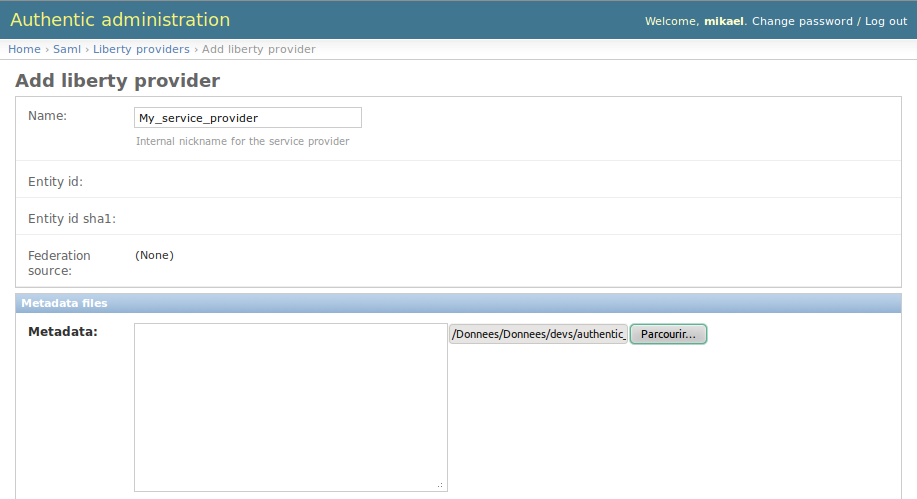
\includegraphics{new_saml2_sp_1.png}

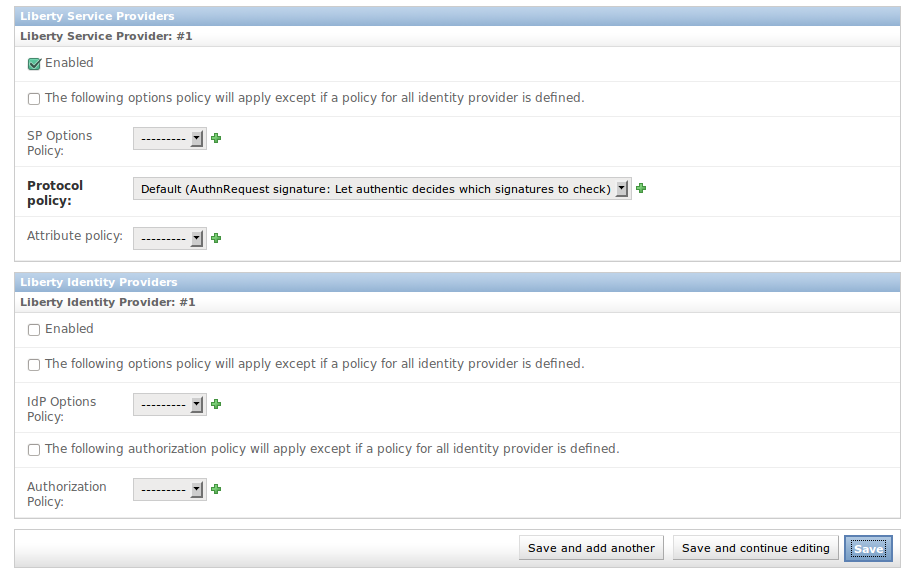
\includegraphics{new_saml2_sp_2.png}

\textbf{The service provider must be enabled.}

See below about configuring the service provider with policies:
\begin{itemize}
\item {} 
options of the service provider

\item {} 
protocol policy

\item {} 
attribute policy

\end{itemize}
\begin{enumerate}
\setcounter{enumi}{2}
\item {} 
Save

\end{enumerate}

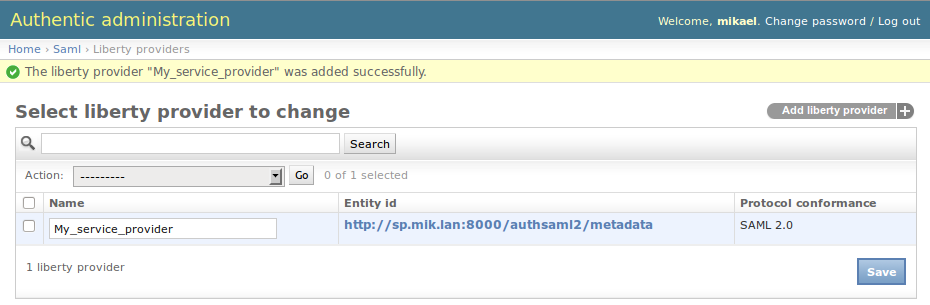
\includegraphics{new_saml2_sp_saved.png}


\subsubsection{Configure the SAML2 service provider options}
\label{config_saml2_sp:configure-the-saml2-service-provider-options}
The SAML2 options of the service provider are configured using sp options
policies.

See the \emph{administration with policy principle} page {\hyperref[administration_with_policies:administration-with-policies]{\emph{How global policies are used in Authentic2 administration}}}.

You may create a regular policy and configure your service provider to use it.

Go to:
\begin{quote}

http{[}s{]}://your.domain.com/admin/saml/spoptionsidppolicy/add/
\end{quote}

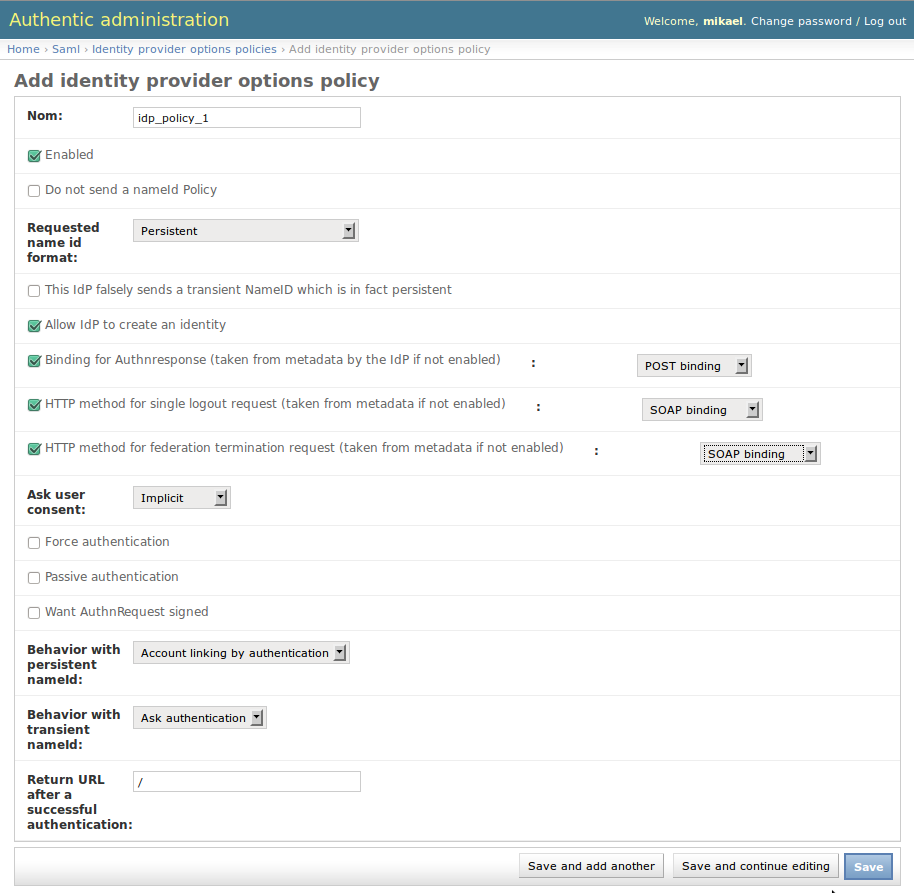
\includegraphics{sp_options_regular.png}

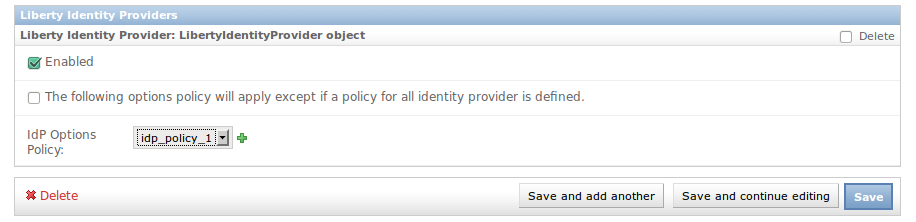
\includegraphics{sp_options_regular_modify_sp.png}

Exemple with a policy `Default':

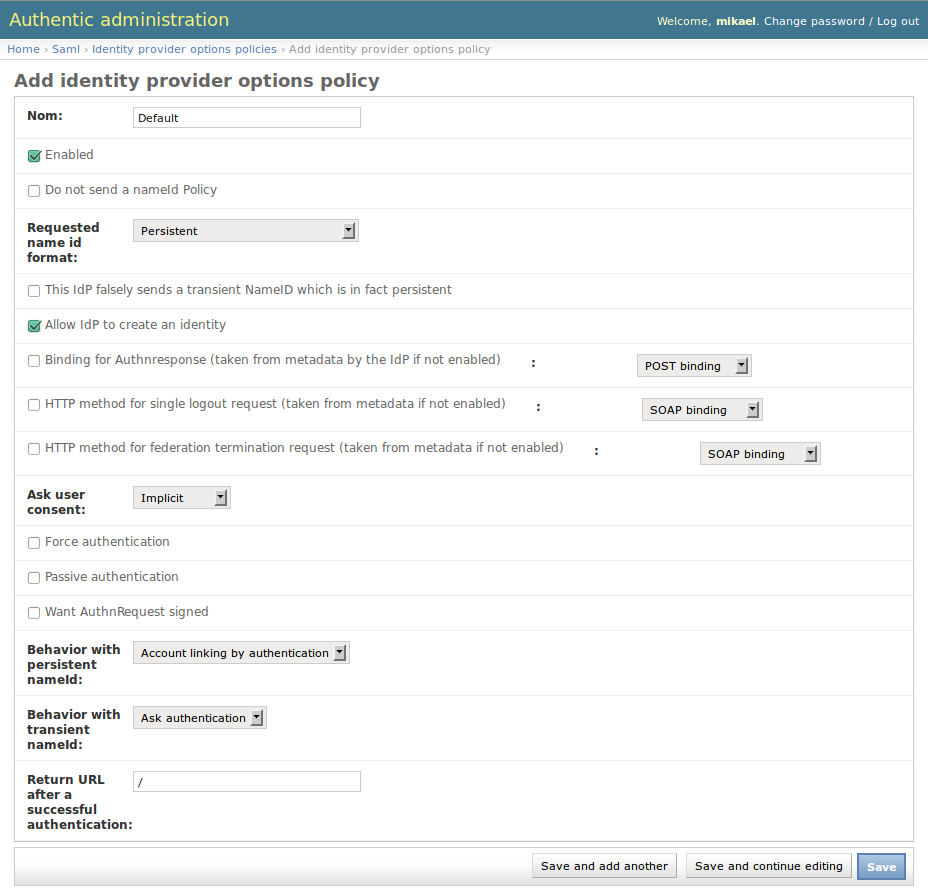
\includegraphics{sp_options_default.png}

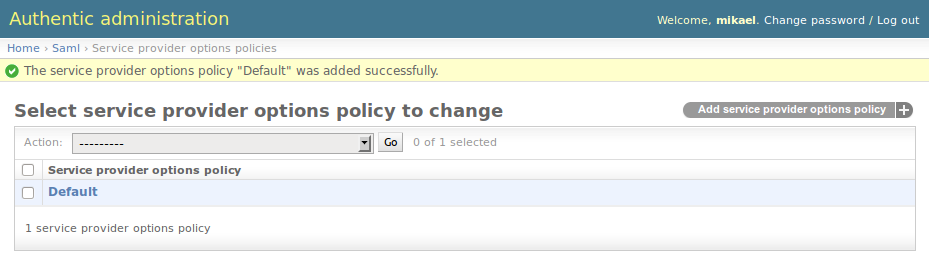
\includegraphics{sp_options_default_saved.png}

Exemple with a policy `All':

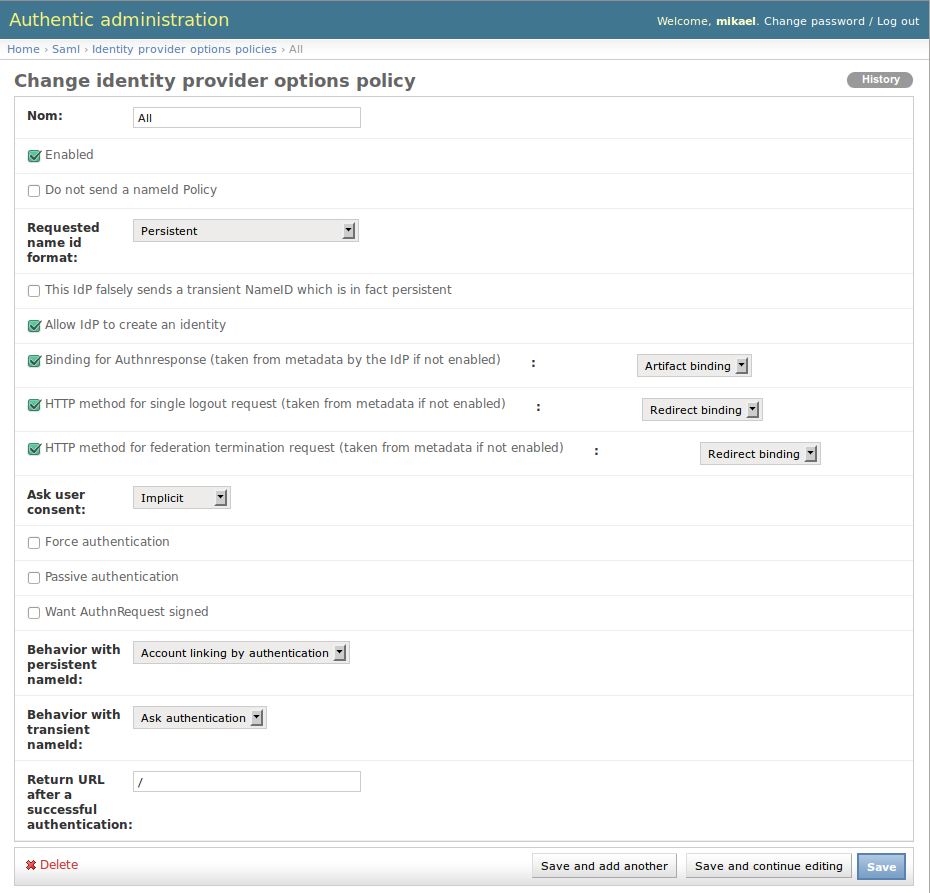
\includegraphics{sp_options_all.png}

If no policy is found for the configuration of the SAML2 options of a service
provider, the following error is displayed when a SSO request is received.

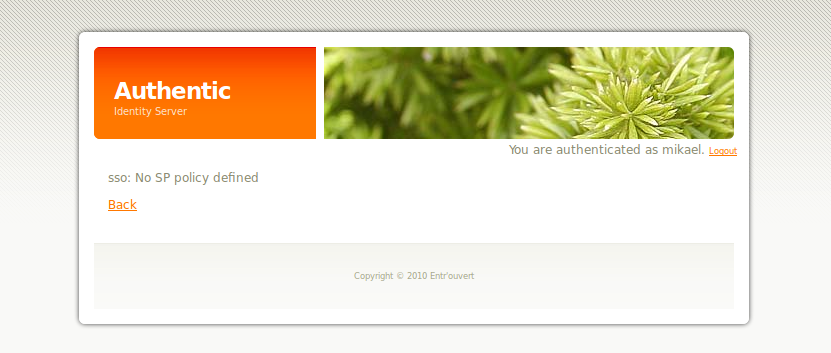
\includegraphics{error_no_sp_options.png}


\subsubsection{Configure the SAML2 service provider protocol options}
\label{config_saml2_sp:configure-the-saml2-service-provider-protocol-options}
This kind of policy does not use the policy management using global policies.

You should use the default option except if your service provider is a
Shibboleth service provider.


\subsubsection{Configure the attribute policy of the service provider}
\label{config_saml2_sp:configure-the-attribute-policy-of-the-service-provider}
See the attribute management page {\hyperref[attribute_management:attribute-management]{\emph{Attribute Management in Authentic2}}}.


\subsubsection{How to refresh metadata of an identity provider hosted at a Well-Known Location?}
\label{config_saml2_sp:how-to-refresh-metadata-of-an-identity-provider-hosted-at-a-well-known-location}
The Well-Known Location (WKL) means that the entity Id of the provider is a
URL at which the provider metadata are hosted.

To refresh them, select the provider on the list of provider, then select in
the menu `Update metadata', then click on `Go'.

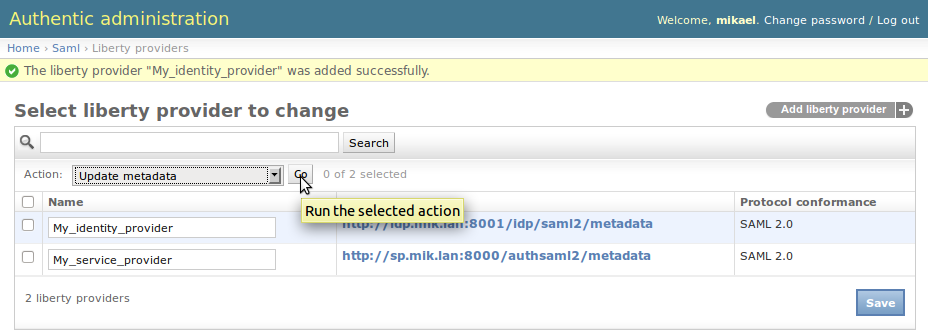
\includegraphics{update_metadata.png}


\subsubsection{How to create in bulk service providers with the sync-metadata script?}
\label{config_saml2_sp:how-to-create-in-bulk-service-providers-with-the-sync-metadata-script}
See the page explaining the use of the script sync-metadata {\hyperref[sync-metadata_script:sync-metadata-script]{\emph{How to create/import and delete in bulk SAML2 identity and service providers with the sync-metadata script?}}}.


\section{Configure Authentic2 as a SAML2 service provider or a SAML2 proxy}
\label{config_saml2_idp:config-saml2-idp}\label{config_saml2_idp::doc}\label{config_saml2_idp:configure-authentic2-as-a-saml2-service-provider-or-a-saml2-proxy}
\textbf{The configuration to make Authentic2 a SAML2 service provider or a SAML2
proxy is the same. The difference comes from that Authentic2 is may be
configured or not as a SAML2 identity provider.}


\subsection{How do I authenticate against a third SAML2 identity provider?}
\label{config_saml2_idp:how-do-i-authenticate-against-a-third-saml2-identity-provider}\begin{enumerate}
\item {} 
Declare Authentic2 as a SAML2 service provider on your SAML2 identity provider using the SAML2 service provider metadata of Authentic2.

\end{enumerate}

Go to http{[}s{]}://your.domain.com/authsaml2/metadata
\begin{enumerate}
\setcounter{enumi}{1}
\item {} 
Add and configure a SAML2 identity provider entry in Authentic2 using the metadata of the identity provider.

\end{enumerate}


\subsection{How do I add and configure a SAML2 identity provider in Authentic2?}
\label{config_saml2_idp:how-do-i-add-and-configure-a-saml2-identity-provider-in-authentic2}
You first need to create a SAML2 identity provider entry with the SAML2
metadata of the identity provider. Then, you configure it.

If your identity provider is Authentic2, the metadata are available at:
\begin{quote}

http{[}s{]}://your.domain.com/idp/saml2/metadata
\end{quote}

See {\hyperref[where_metadata:where-metadata]{\emph{Where do I find the Authentic2 SAML2 metadata?}}} for more information.


\subsubsection{Create a SAML2 identity provider entry}
\label{config_saml2_idp:create-a-saml2-identity-provider-entry}
You first need to create a new SAML2 identity provider entry. This requires
the SAML2 metadata of the identity provider.
\begin{enumerate}
\item {} 
Go to
\begin{quote}

http{[}s{]}://your.domain.com/admin/saml/libertyprovider/add/
\end{quote}

\item {} 
Fill the form fields

\end{enumerate}

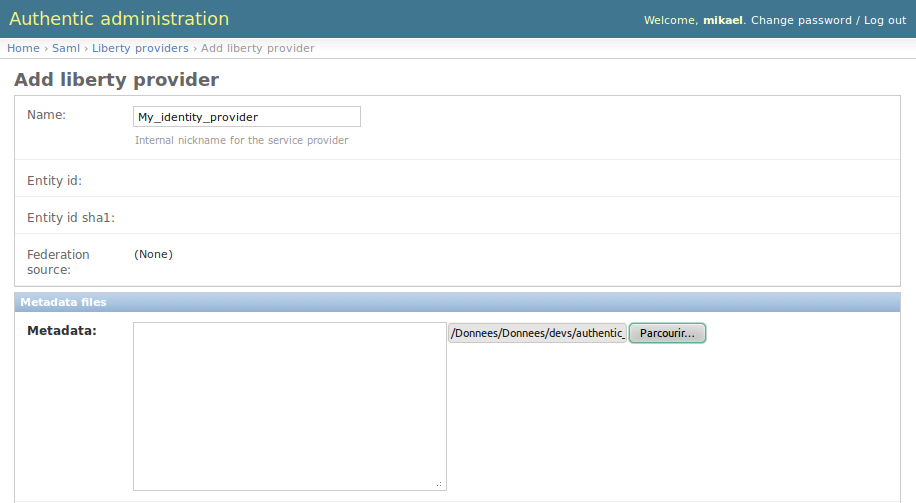
\includegraphics{new_saml2_idp_1.png}

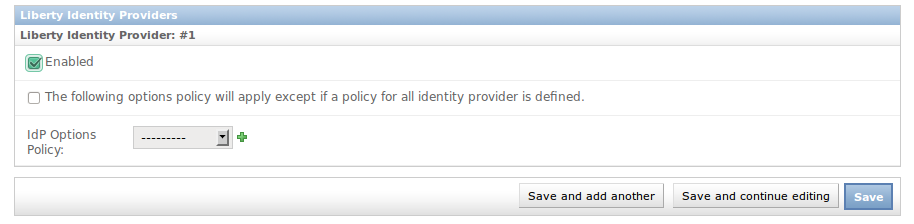
\includegraphics{new_saml2_idp_2.png}

\textbf{The identity provider must be enabled.}

See below about configuring the identity provider with policies:
\begin{itemize}
\item {} 
options of the identity provider

\end{itemize}
\begin{enumerate}
\setcounter{enumi}{2}
\item {} 
Save

\end{enumerate}

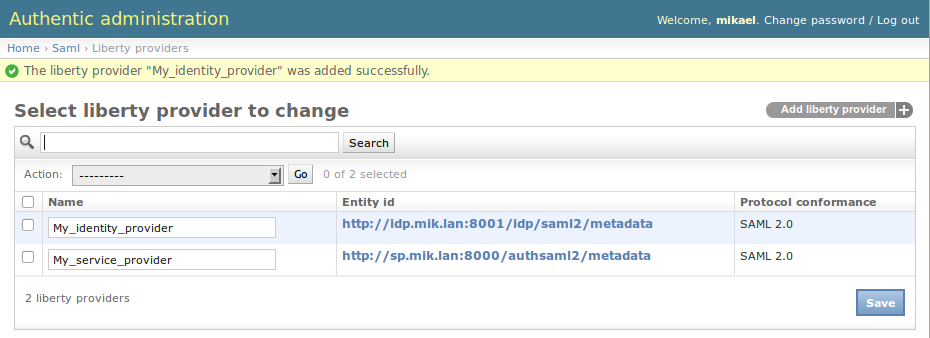
\includegraphics{new_saml2_idp_saved.png}


\subsubsection{Configure the SAML2 identity provider options}
\label{config_saml2_idp:configure-the-saml2-identity-provider-options}
The SAML2 options of the service provider are configured using sp options
policies.

See the \emph{administration with policy principle} page {\hyperref[administration_with_policies:administration-with-policies]{\emph{How global policies are used in Authentic2 administration}}}.

You may create a regular policy and configure your service provider to use it.

Go to:
\begin{quote}

http{[}s{]}://your.domain.com/admin/saml/idpoptionssppolicy/add/
\end{quote}

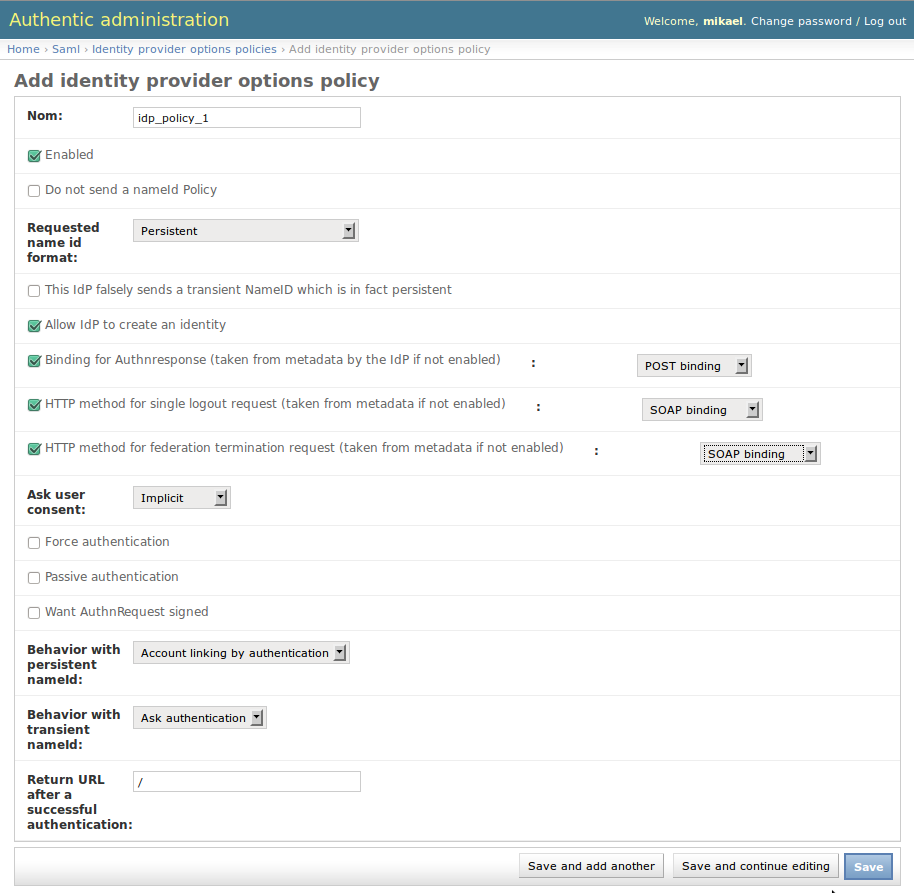
\includegraphics{sp_options_regular.png}

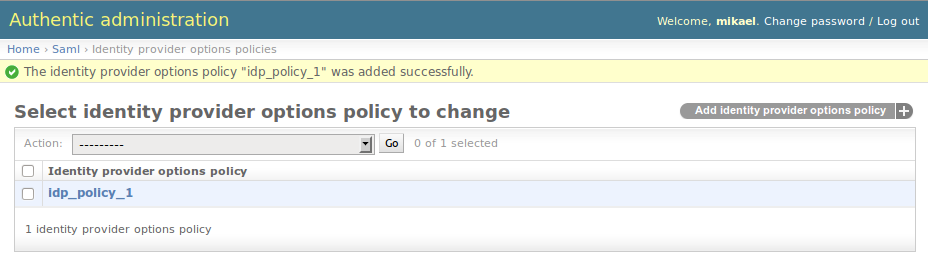
\includegraphics{sp_options_regular_saved.png}

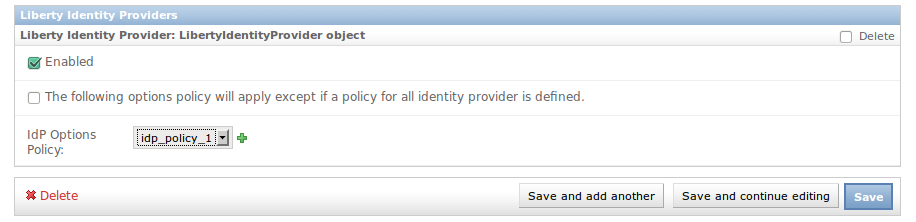
\includegraphics{sp_options_regular_modify_sp.png}

Exemple with a policy `Default':

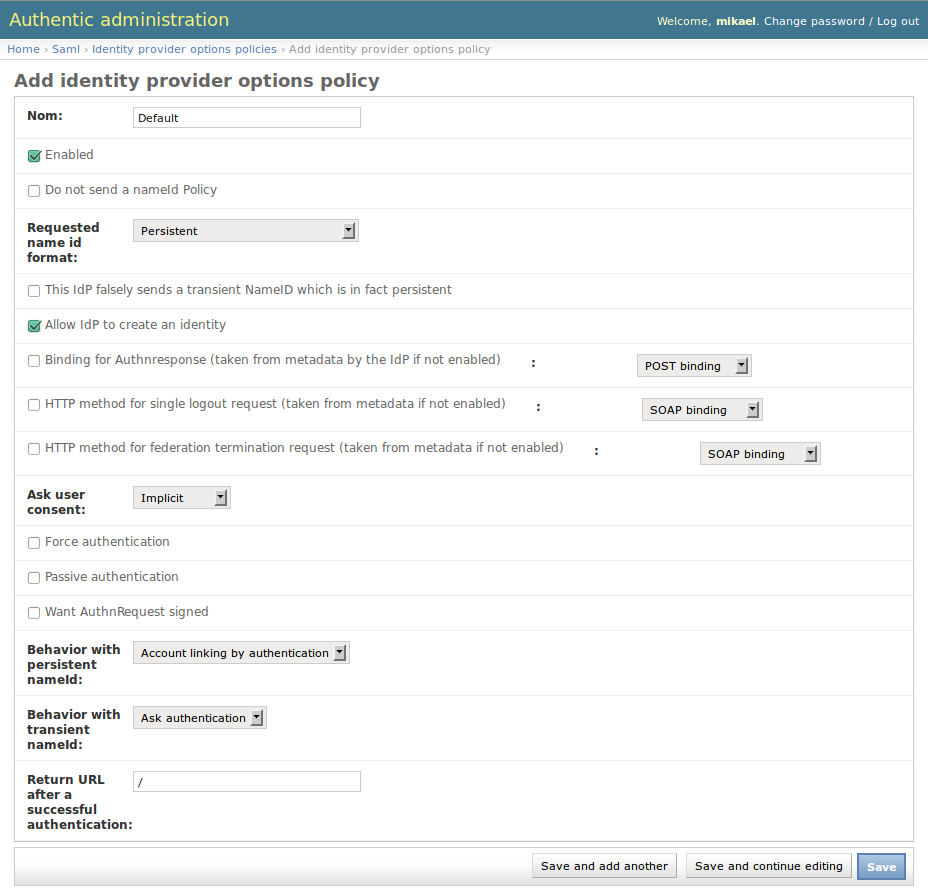
\includegraphics{sp_options_default.png}

Exemple with a policy `All':

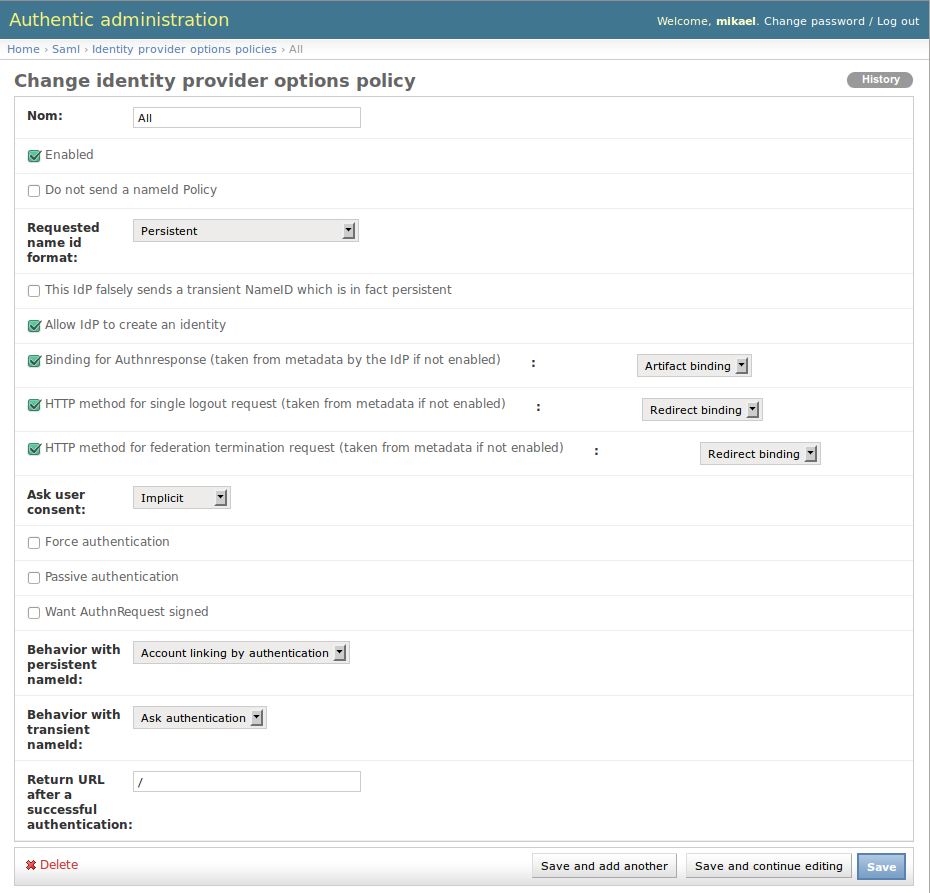
\includegraphics{sp_options_all.png}

If no policy is found for the configuration of the SAML2 options of an identity
provider, the following error is displayed when a SSO request is initiated.

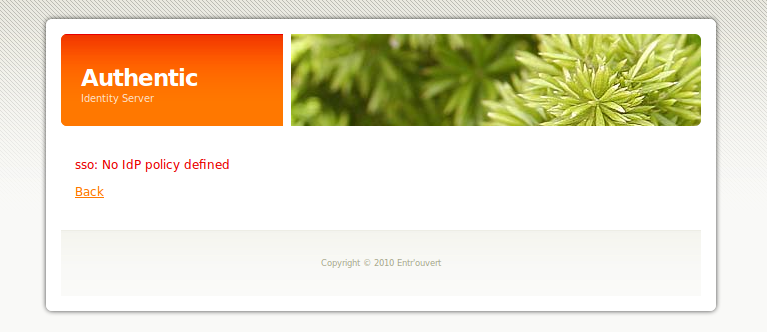
\includegraphics{error_no_idp_options.png}


\subsubsection{How to refresh metadata of an identity provider hosted at a Well-Known Location?}
\label{config_saml2_idp:how-to-refresh-metadata-of-an-identity-provider-hosted-at-a-well-known-location}
The Well-Known Location (WKL) means that the entity Id of the provider is a
URL at which the provider metadata are hosted.

To refresh them, select the provider on the list of provider, then select in
the menu `Update metadata', then click on `Go'.

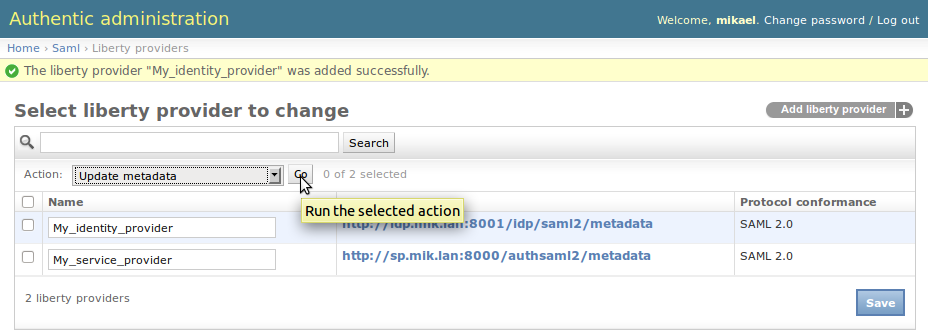
\includegraphics{update_metadata.png}

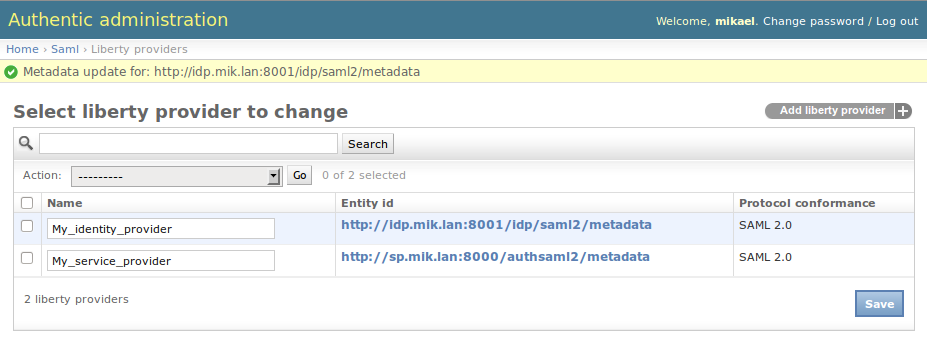
\includegraphics{update_metadata_done.png}


\subsubsection{How to create in bulk identity providers with the sync-metadata script?}
\label{config_saml2_idp:how-to-create-in-bulk-identity-providers-with-the-sync-metadata-script}
See the page explaining the use of the script sync-metadata {\hyperref[sync-metadata_script:sync-metadata-script]{\emph{How to create/import and delete in bulk SAML2 identity and service providers with the sync-metadata script?}}}.


\section{How to create/import and delete in bulk SAML2 identity and service providers with the sync-metadata script?}
\label{sync-metadata_script:how-to-create-import-and-delete-in-bulk-saml2-identity-and-service-providers-with-the-sync-metadata-script}\label{sync-metadata_script:sync-metadata-script}\label{sync-metadata_script::doc}
This section explains hot to use the script sync-metadata.


\subsection{Presentation}
\label{sync-metadata_script:presentation}
This script allows to create/import and deleted in bulk SAML2 identity and
service providers using standard SAML2 metadata files containing entity
descriptors.

An example of such a file used in production is the global metadata file of
the identity federation of French universities that can be found at \href{http://}{http://}...

Use the following command:

\begin{Verbatim}[commandchars=\\\{\}]
path\_to\_project/authentic2\$ python manage.py sync-metadata file\_name [options]
\end{Verbatim}


\subsection{Options}
\label{sync-metadata_script:options}\begin{itemize}
\item {} 
idp
\begin{quote}

Load only identity providers of the metadata file.
\end{quote}

\item {} 
sp
\begin{quote}

Load only service providers of the metadata file.
\end{quote}

\item {} 
source
\begin{quote}

Used to tag all imported providers with a label. This option is used to
metadata reloading and deletion in bulk.

Reloading a metadata file, when a provider with same entity is found, it is
updated. If a provider in the metadata file does not exist it is created.
If a provider exists in the system but not in the metadata file, it is
removed.

\textbf{For reloading, a source can only be associated with a unique metadata
file. This is due to the fact that all providers of a source not found in
the metadata file are removed.}
\end{quote}

\end{itemize}

\begin{Verbatim}[commandchars=\\\{\}]
path\_to\_project/authentic2\$ python manage.py sync-metadata file\_name --source=french\_federation
\end{Verbatim}
\begin{itemize}
\item {} 
sp-policy
\begin{quote}

To configure the SAML2 parameters of service providers imported with the
script, a policy of type SPOptionsIdPPolicy must be created in the
the administration interface.
Either it is a global policy `Default' or `All' or it is a regular policy.
If it is a regular policy, the policy name can be specified in parameter
of the script with this option.
The policy is then associated to all service providers created.
\end{quote}

\end{itemize}

\begin{Verbatim}[commandchars=\\\{\}]
path\_to\_project/authentic2\$ python manage.py sync-metadata file\_name --sp-policy=sp\_policy\_name
\end{Verbatim}
\begin{itemize}
\item {} 
idp-policy
\begin{quote}

To configure the SAML2 parameters of identity providers imported with the
script, a policy of type IdPOptionsSPPolicy must be created in the
the administration interface.
Either it is a global policy `Default' or `All' or it is a regular policy.
If it is a regular policy, the policy name can be specified in parameter
of the script with this option.
The policy is then associated to all service providers created.
\end{quote}

\end{itemize}

\begin{Verbatim}[commandchars=\\\{\}]
path\_to\_project/authentic2\$ python manage.py sync-metadata file\_name --idp-policy=idp\_policy\_name
\end{Verbatim}
\begin{itemize}
\item {} 
delete
\begin{quote}

With no options, all providers are deleted.

With the source option, only providers with the source name given are deleted.

\textbf{This option can not be combined with options idp and sp.}
\end{quote}

\item {} 
ignore-errors
\begin{quote}

If loading of one EntityDescriptor fails, continue loading
\end{quote}

\end{itemize}


\section{Configure Authentic2 as a CAS server}
\label{config_cas_sp:configure-authentic2-as-a-cas-server}\label{config_cas_sp::doc}\label{config_cas_sp:config-cas-sp}

\subsection{How to use Authentic2 as a CAS 1.0 or CAS 2.0 identity provider ?}
\label{config_cas_sp:how-to-use-authentic2-as-a-cas-1-0-or-cas-2-0-identity-provider}\begin{enumerate}
\item {} 
Activate CAS IdP support in settings.py:

\begin{Verbatim}[commandchars=\\\{\}]
\PYG{n}{IDP\PYGZus{}CAS} \PYG{o}{=} \PYG{n+nb+bp}{True}
\end{Verbatim}

\item {} 
Then create the database table to hold CAS service tickets:

\begin{Verbatim}[commandchars=\\\{\}]
python authentic2/manage.py syncdb --migrate
\end{Verbatim}

\item {} 
Also configure authentic2 to authenticate against your LDAP directory (see
above) if your want your user attributes to be accessible from your service,
if it is not necessary you can use the normal relational database storage
for you users.

\item {} 
Finally configure your service to point to the CAS endpoint at:
\begin{quote}

http{[}s{]}://your.domain.com/idp/cas/
\end{quote}

\item {} 
If needed configure your service to resolve authenticated user with your
LDAP directory (if user attributes are needed for your service)

\end{enumerate}


\section{Configure Authentic2 as a CAS client}
\label{config_cas_idp::doc}\label{config_cas_idp:configure-authentic2-as-a-cas-client}\label{config_cas_idp:config-cas-idp}

\section{Attribute Management in Authentic2}
\label{attribute_management:attribute-management}\label{attribute_management:attribute-management-in-authentic2}\label{attribute_management::doc}

\subsection{Summary}
\label{attribute_management:summary}
Attribute management currently allows to configure attribute policies
associated with SAML2 service providers to define attributes that are
pushed in SAML2 successful authentication response delivered by Authentic2.

User attributes can be taken from LDAP directories, the user Django
profile or taken from the user Django session if Authentic2 is also configured
as a SAML2 service provider.

Indeed, when Authentic2 acts also as a SAML2 service provider,
attributes contained in the SAML2 assertion received from third IdP are put in
the user session.

Attributes can thus be proxyfied during SSO with Authentic2
configured as a SAML2 proxy.

The namespace of attributes received from another SAML2 IdP or pushed in the
assertion given in to service providers can be configured per attribute or per
service provider.

By default, the namespace and format of attributes in assertion is conformant
to the SAMLV2.0 X500/LDAP Attribute profile:

\begin{Verbatim}[commandchars=\\\{\}]
\textless{}saml:Attribute
    xmlns:x500="urn:oasis:names:tc:SAML:2.0:profiles:attribute:X500"
    NameFormat="urn:oasis:names:tc:SAML:2.0:attrname-format:uri"
    Name="urn:oid:2.5.4.42" FriendlyName="givenName"\textgreater{}
    \textless{}saml:AttributeValue xsi:type="xs:string"
        x500:Encoding="LDAP"\textgreater{}Mikaël\textless{}/saml:AttributeValue\textgreater{}
\textless{}/saml:Attribute\textgreater{}
\end{Verbatim}

But the \href{http://schemas.xmlsoap.org/ws/2005/05/identity/claims}{http://schemas.xmlsoap.org/ws/2005/05/identity/claims} from the ISI
profile can also be used, for instance:

\begin{Verbatim}[commandchars=\\\{\}]
\textless{}saml:Attribute
    NameFormat="urn:oasis:names:tc:SAML:2.0:attrname-format:uri"
    Name="http://schemas.xmlsoap.org/ws/2005/05/identity/claims/givenname"
    FriendlyName="First Name"\textgreater{}
    \textless{}saml:AttributeValue\textgreater{}Mikaël\textless{}/saml:AttributeValue\textgreater{}
\textless{}/saml:Attribute\textgreater{}
\end{Verbatim}


\subsection{Configuration}
\label{attribute_management:configuration}

\subsubsection{Configure sources of attributes}
\label{attribute_management:configure-sources-of-attributes}
The source of attributes for authentic2 are of two kinds. The LDAP sources and
the user django profile.


\paragraph{Declare the Django profile source}
\label{attribute_management:declare-the-django-profile-source}
Add an attribute source named USER\_PROFILE with namespace `Default'.
\begin{enumerate}
\item {} 
Go to http{[}s{]}://your.domain.com/admin/attribute\_aggregator/attributesource/add/

\item {} 
Write `USER\_PROFILE' in name field

\end{enumerate}

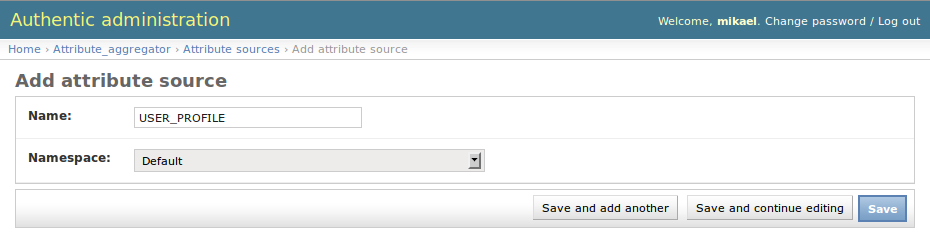
\includegraphics{user_profile_source.png}
\begin{enumerate}
\setcounter{enumi}{2}
\item {} 
Save

\end{enumerate}

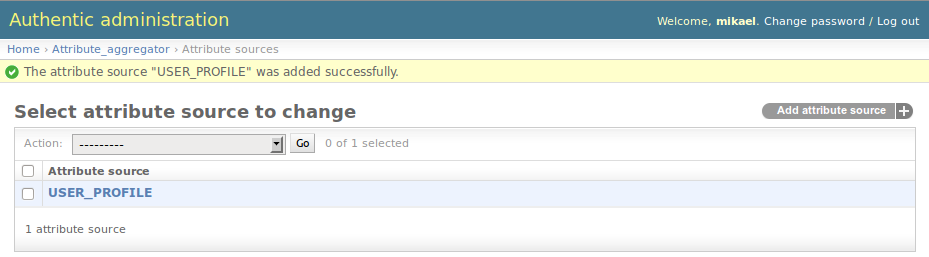
\includegraphics{user_profile_source_saved.png}


\paragraph{Add an LDAP Source}
\label{attribute_management:add-an-ldap-source}
For LDAP sources, objects of type `LDAPSource' must be created.

\textbf{Even if the authentication is based on LDAP authentification, thus that a
server is configured in settings.py, it is
necessary to create a corresponding `LDAPSource' to use it as a source of
attribute.}
\begin{enumerate}
\item {} 
Go to http{[}s{]}://your.domain.com/admin/attribute\_aggregator/ldapsource/add/

\item {} 
Fill form fields

\end{enumerate}

Only the field Name, Server, User, Password, Base and Port are used for now.
\textbf{The namespace of LDAP source must be kept to `Default', since the system
namespace is based on LDAP.}

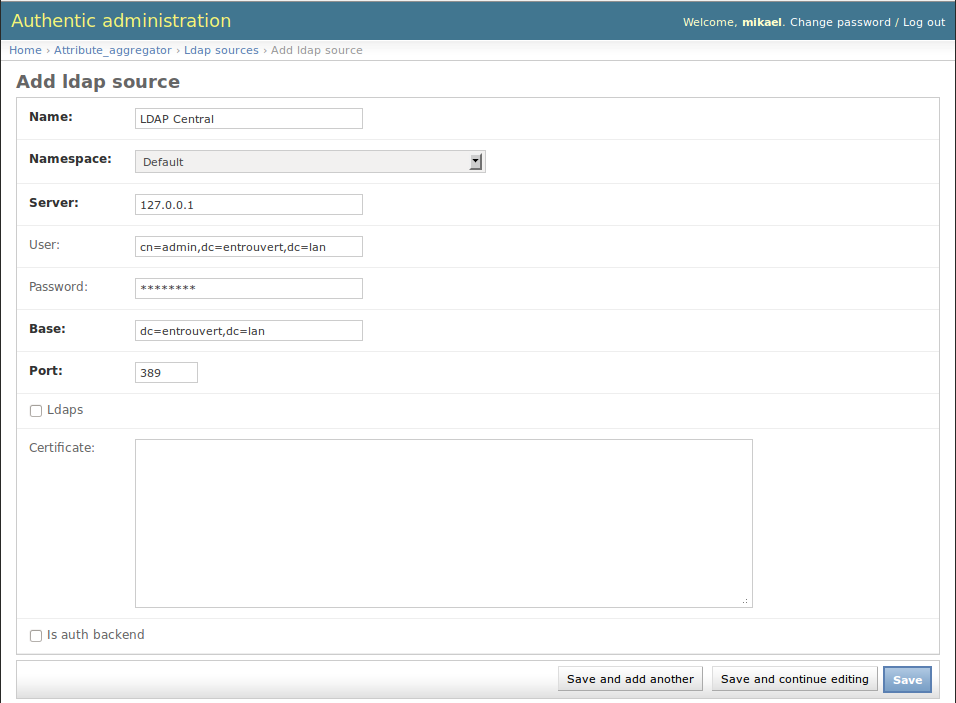
\includegraphics{ldapsource.png}
\begin{enumerate}
\setcounter{enumi}{2}
\item {} 
Save

\end{enumerate}

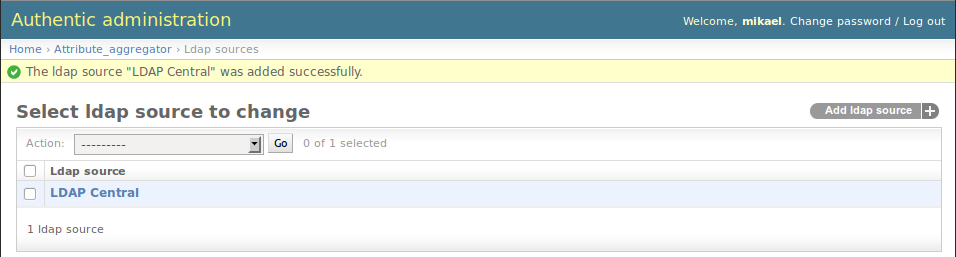
\includegraphics{ldapsource_saved.png}


\paragraph{Manage user distinguished names in LDAP directories}
\label{attribute_management:manage-user-distinguished-names-in-ldap-directories}
To find the user in a LDAP directory, authentic2 must know its distinguished
name (DN). If this LDAP has been used when the user has authenticated,
Authentic2 learn the user DN. Nothing has to be done from this point of view.

However, if it is expected that user attributes be taken in a directory that
is not used by the user for authentication, it is necessary to manually
indicate to Authentic2 what is the user DN in the directory. For this, a
user alias in source is created for the user:
\begin{enumerate}
\item {} 
Go to http{[}s{]}://your.domain.com/admin/attribute\_aggregator/useraliasinsource/add/

\item {} 
Fill form fields

\end{enumerate}

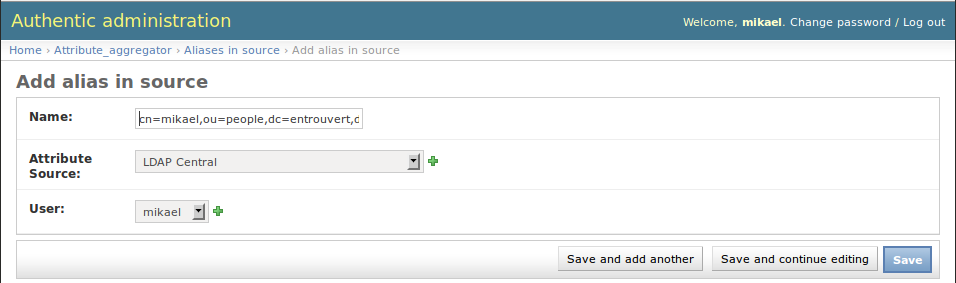
\includegraphics{alias_in_source.png}
\begin{enumerate}
\setcounter{enumi}{2}
\item {} 
Save

\end{enumerate}

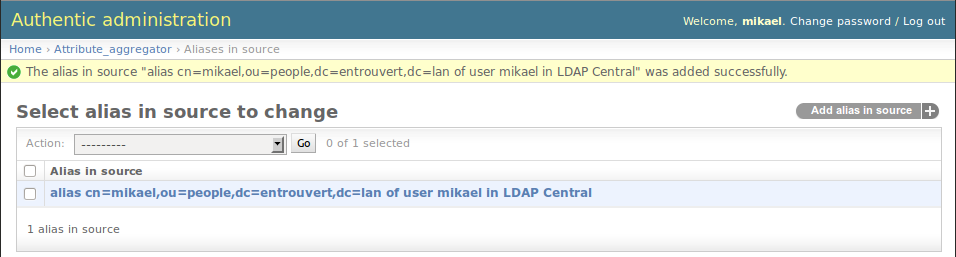
\includegraphics{alias_in_source_saved.png}


\subsubsection{Configure attributes pushed to SAML2 service providers in SSO response}
\label{attribute_management:configure-attributes-pushed-to-saml2-service-providers-in-sso-response}
Reminder:
\begin{itemize}
\item {} 
The default name format in SAML2 assertions is URI

\item {} 
The default namespace called `Default' is LDAP

\end{itemize}

In summary:
\begin{enumerate}
\item {} 
Create attribute items indicating an attribute name, a source, the name format expected and the namespace expected for the attribute name and friendly name if any.

\item {} 
Create a named list of attribute items.

\item {} 
Create an attribute policy and associate the previous list or associate the previous list to a existing attribute policy.

\item {} 
Associate the policy to a service provider.

\end{enumerate}


\paragraph{Create attribute items}
\label{attribute_management:create-attribute-items}\begin{enumerate}
\item {} 
Go to http{[}s{]}://your.domain.com/admin/idp/attributeitem/add/

\item {} 
Fill form fields

\end{enumerate}

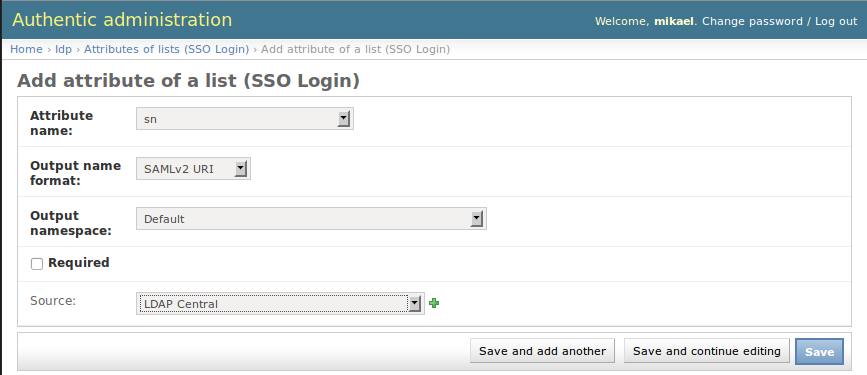
\includegraphics{attribute_item.png}
\begin{enumerate}
\setcounter{enumi}{2}
\item {} 
Save

\end{enumerate}

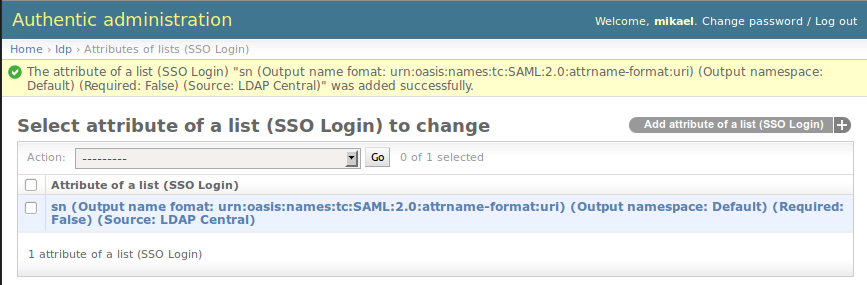
\includegraphics{attribute_item_saved.png}


\paragraph{Create a named list of attribute items}
\label{attribute_management:create-a-named-list-of-attribute-items}\begin{enumerate}
\item {} 
Go to http{[}s{]}://your.domain.com/admin/idp/attributelist/add/

\item {} 
Name the list and add items to list

\end{enumerate}

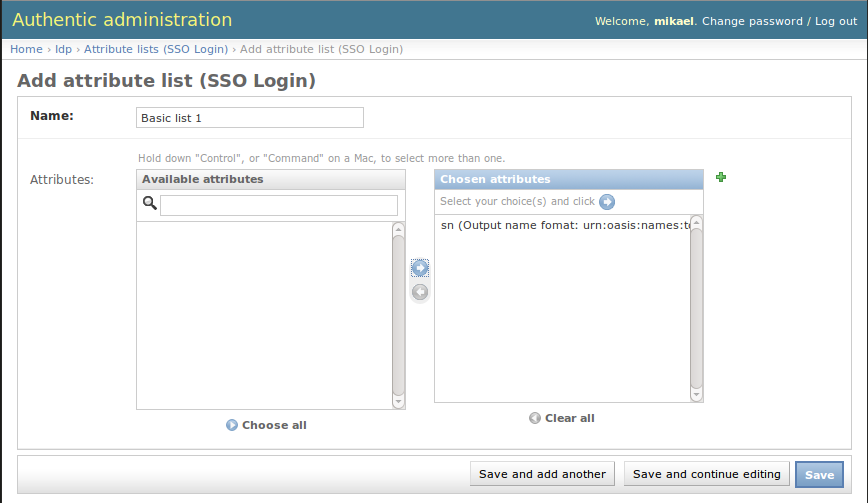
\includegraphics{attribute_list.png}
\begin{enumerate}
\setcounter{enumi}{2}
\item {} 
Save

\end{enumerate}

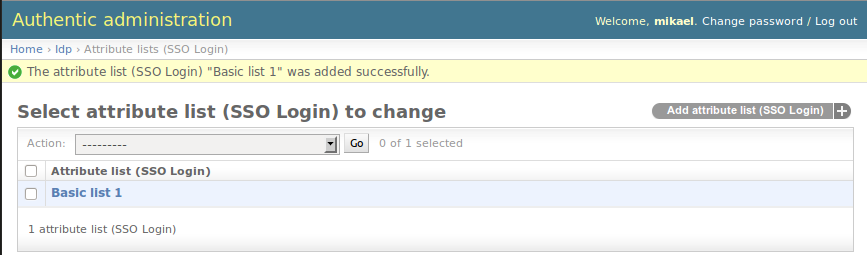
\includegraphics{attribute_list_saved.png}


\paragraph{Create or modify an attribute policy}
\label{attribute_management:create-or-modify-an-attribute-policy}\begin{enumerate}
\item {} 
Go to http{[}s{]}://your.domain.com/admin/idp/attributepolicy/add/

\item {} 
Add list to the policy

\end{enumerate}

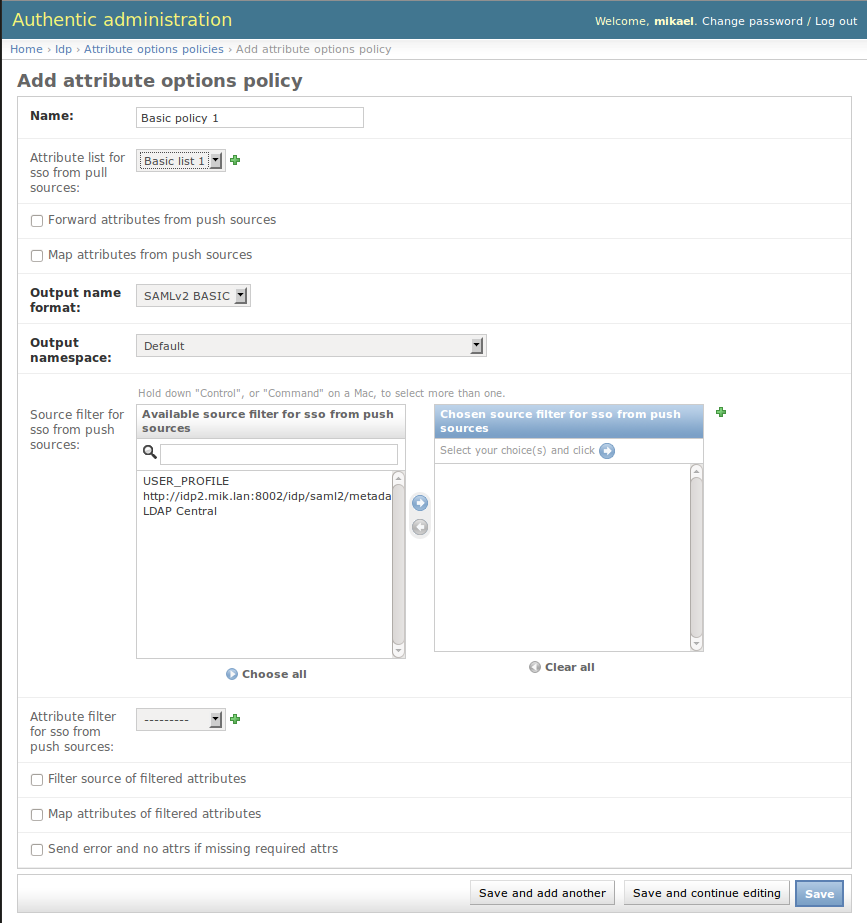
\includegraphics{policy_pull.png}
\begin{enumerate}
\setcounter{enumi}{2}
\item {} 
Save

\end{enumerate}

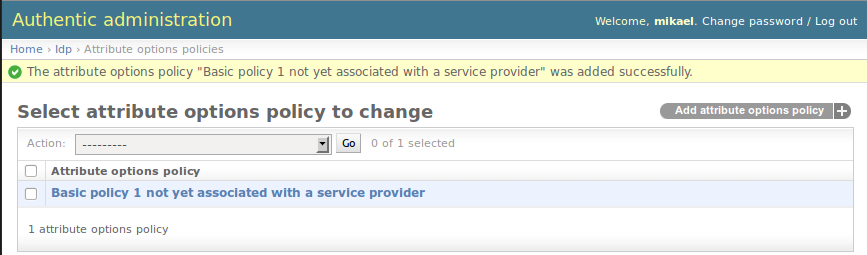
\includegraphics{policy_pull_saved.png}


\paragraph{Associate the policy to a service provider}
\label{attribute_management:associate-the-policy-to-a-service-provider}\begin{enumerate}
\item {} 
Go to http{[}s{]}://your.domain.com/admin/saml/libertyprovider/1/

\item {} 
Add policy to the service provider

\end{enumerate}

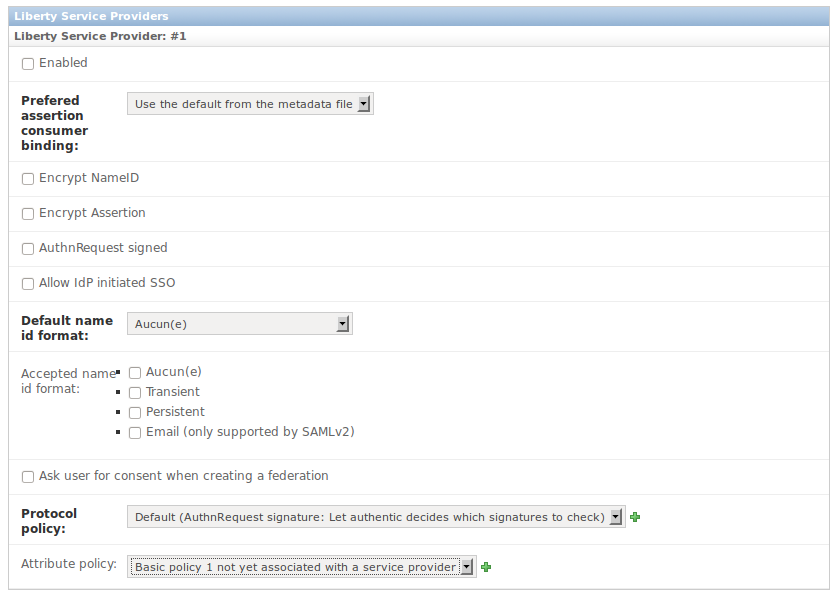
\includegraphics{sp_policy_pull.png}
\begin{enumerate}
\setcounter{enumi}{2}
\item {} 
Save

\end{enumerate}

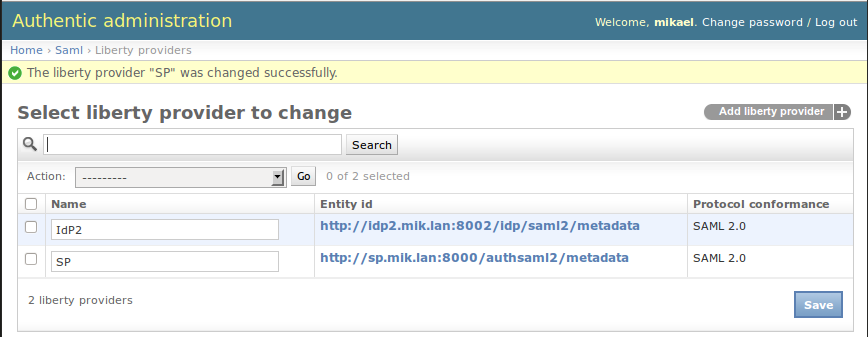
\includegraphics{sp_policy_pull_saved.png}
\begin{enumerate}
\setcounter{enumi}{3}
\item {} 
The display name of the policy has changed

\end{enumerate}

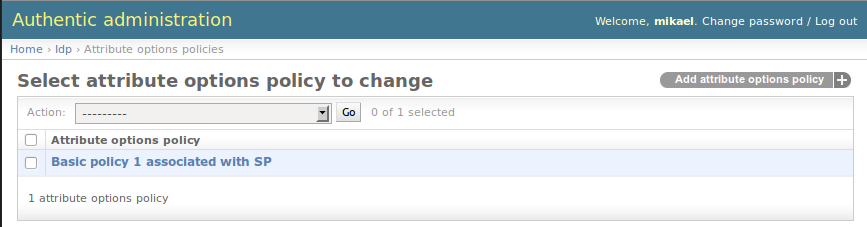
\includegraphics{policy_pull_renamed.png}


\subsubsection{Handle attributes provided by other Identity providers, proxy attributes}
\label{attribute_management:handle-attributes-provided-by-other-identity-providers-proxy-attributes}
Link to configure first Authentic as a sp to have attributes in session

Add a source if mapping set to true


\subsection{Modifying supported namespaces and attribute name mappings}
\label{attribute_management:modifying-supported-namespaces-and-attribute-name-mappings}
TBD


\subsection{Explanation (Draft)}
\label{attribute_management:explanation-draft}

\subsubsection{Attribute aggegrator module}
\label{attribute_management:attribute-aggegrator-module}
The core attribute management is based on the attribute aggregator module.


\paragraph{Intro}
\label{attribute_management:intro}
Attribute aggregator provides a main Model class called UserAttributeProfile,
functions to load attributes and extract attributes.

The mapping between attribute namespaces is built-in and depends on a unique
file (mapping.py).

A main schema is defined and is based on LDAP/X500 for naming. The support
of \href{http://schemas.xmlsoap.org/ws/2005/05/identity/claims}{http://schemas.xmlsoap.org/ws/2005/05/identity/claims} is partly complete.

Source of attributes are connected with attribute loading functions using
signals.


\paragraph{FAQ}
\label{attribute_management:faq}
Why not use the Django User profile?

The django user profile needs to define attributes as class attributes and
then support form filling or mapping with LDAP.

That is useful and may be used, especially because the profile can be used as
a source of attribute to load in the attribute\_aggregator profile.

The attribute\_aggregator profile allow to load multivalued attributes from any
source supported (LDAP, Django profile and attributes in Django session for
now) from any namespace defined in mapping.py (LDAP/X500 and claims for now).

The profile can be loaded giving a source or a list of attribute, or can be
from any known source, or with a dictionnary.

Attributes can be extracted with many functions in any namespace supported.


\paragraph{Quick explanation}
\label{attribute_management:quick-explanation}
The schema is defined in mapping.py and is made of definitions like this:

\begin{Verbatim}[commandchars=\\\{\}]
"sn": \PYGZob{}
    "oid": "2.5.4.4",
    "display\_name": \_("sn surname"),
    "alias": ['surname'],
    "profile\_field\_name": 'last\_name',
    "type": "http://www.w3.org/2001/XMLSchema\#string",
    "namespaces": \PYGZob{}
        "http://schemas.xmlsoap.org/ws/2005/05/identity/claims": \PYGZob{}
            "identifiers":
                [
        "http://schemas.xmlsoap.org/ws/2005/05/identity/claims/surname",
                ],
            "friendly\_names":
                [
            "Last Name",
                ],
        \PYGZcb{}
    \PYGZcb{}
\PYGZcb{},
\end{Verbatim}

The profile store all the data in a text field taht contains a cPickle list of
instances of the class AttributeData.

The profile is attached to a user and then can be created or loaded with:

\begin{Verbatim}[commandchars=\\\{\}]
\PYG{n}{profile} \PYG{o}{=} \PYG{n}{load\PYGZus{}or\PYGZus{}create\PYGZus{}user\PYGZus{}profile}\PYG{p}{(}\PYG{n}{user}\PYG{o}{=}\PYG{n}{user}\PYG{p}{)}
\end{Verbatim}

User may be None to create a temporary profile for an anonymous user. But
that need a DB cleaning function not implemented.


\paragraph{The model \emph{UserAttributeProfile}}
\label{attribute_management:the-model-userattributeprofile}
The model `UserAttributeProfile' can be attached to a user and then persist
(as a Model).

When the profile is loaded, all data stored are removed expect if the
the data has an expiration date later.

The profile provide several methods to store and extract attributes.

All the methods to add attributes are based on a main one accepting a
dictionnary of attribute is parameters `load\_by\_dic()'. The other methods
(`load\_listed\_attributes()', `load\_greedy()') send a signal with a list of
attributes (listed\_attributes\_call) or not (any\_attributes\_call) to grab a
dictionnary. The list is given with the definition name, oid or friendly name
of the attribute in the system namespace.

Into the dictionnary, attributes are given with their name, oid or friendly
name in the default namespace or with their name in a namepsace. An expiration
date can also be given (ISO8601 format), if none, attribute will be deleted at
next profile loading. The dictionnary format is as follows:

\begin{Verbatim}[commandchars=\\\{\}]
attributes = dict()
data\_from\_source = list()
a1 = dict()
    a1['oid'] = definition\_name
Or
    a1['definition'] = definition\_name
        definition may be the definition name like 'gn'
        or an alias like 'givenName'
Or
    a1['name'] = attribute\_name\_in\_ns
    a1['namespace'] = ns\_name
a1['expiration\_date'] = date
a1['values'] = list\_of\_values
data\_from\_source.append(a1)
...
data\_from\_source.append(a2)
attributes[source\_name] = data\_from\_source
\end{Verbatim}

Getters are defined to extract data from a profile. Only AttributeData
instances are extracted that assume that any attribute namespace can be used.
\begin{itemize}
\item {} 
get\_data\_of\_definition(definition)

\end{itemize}

Return a list of AttributeData instances corresponding to the definition
given.
\begin{itemize}
\item {} 
get\_freshest\_data\_of\_definition(definition)

\end{itemize}

Return the freshest AttributeData instance. If multiple with no or same exp
date, random. Should use the creation date soon.
\begin{itemize}
\item {} 
get\_data\_of\_source

\end{itemize}

Return a list of AttributeData instances corresponding to the source given.
\begin{itemize}
\item {} 
get\_data\_of\_source\_by\_name

\end{itemize}

Idem but source name is given, not a Source instance.
\begin{itemize}
\item {} 
get\_data\_of\_definition\_and\_source

\end{itemize}

Return a list of AttributeData instances corresponding to the definition and
source given.
\begin{itemize}
\item {} 
get\_data\_of\_definition\_and\_source\_by\_name

\end{itemize}

Idem but source name is given, not a Source instance.


\subsubsection{SAML2 attribute representation in assertions}
\label{attribute_management:saml2-attribute-representation-in-assertions}
SAML2 attribute profile (saml-profiles-2.0-os - Section 8) defines two kind of
attribute element syntax in the attribute statement of assertions, also
called \emph{name format}:
\begin{itemize}
\item {} 
BASIC:

\begin{Verbatim}[commandchars=\\\{\}]
\PYG{n}{NameFormat}\PYG{o}{=}\PYG{l+s}{"}\PYG{l+s}{urn:oasis:names:tc:SAML:2.0:attrname-format:basic}\PYG{l+s}{"}
\end{Verbatim}

\item {} 
URI:

\begin{Verbatim}[commandchars=\\\{\}]
\PYG{n}{NameFormat}\PYG{o}{=}\PYG{l+s}{"}\PYG{l+s}{urn:oasis:names:tc:SAML:2.0:attrname-format:uri}\PYG{l+s}{"}
\end{Verbatim}

\end{itemize}

\emph{URI should be used when attributes have ``universally'' known unique names
like OID.}

Example:

\begin{Verbatim}[commandchars=\\\{\}]
\textless{}saml:Attribute NameFormat="urn:oasis:names:tc:SAML:2.0:attrname-format:basic"
    Name="FirstName"\textgreater{}
    \textless{}saml:AttributeValue xsi:type="xs:string"\textgreater{}By-Tor\textless{}/saml:AttributeValue\textgreater{}
\textless{}/saml:Attribute\textgreater{}

\textless{}saml:Attribute
    xmlns:x500="urn:oasis:names:tc:SAML:2.0:profiles:attribute:X500"
    NameFormat="urn:oasis:names:tc:SAML:2.0:attrname-format:uri"
    Name="urn:oid:2.5.4.42" FriendlyName="givenName"\textgreater{}
    \textless{}saml:AttributeValue xsi:type="xs:string"
        x500:Encoding="LDAP"\textgreater{}Steven\textless{}/saml:AttributeValue\textgreater{}
\textless{}/saml:Attribute\textgreater{}
\end{Verbatim}


\paragraph{BASIC}
\label{attribute_management:basic}
Two \textless{}Attribute\textgreater{} elements refer to the same SAML attribute if and only if the
values of their Name XML attributes are equal in the sense of Section 3.3.6 of
{[}Schema2{]}.

No additional XML attributes are defined for use with the \textless{}Attribute\textgreater{} element.

The schema type of the contents of the \textless{}AttributeValue\textgreater{} element MUST be drawn
from one of the types defined in Section 3.3 of {[}Schema2{]}. The xsi:type
attribute MUST be present and be given the appropriate value.


\paragraph{X.500/LDAP Attribute Profile (URI)}
\label{attribute_management:x-500-ldap-attribute-profile-uri}
\textbf{Extracted from the SAML2 core specifications}

Two \textless{}Attribute\textgreater{} elements refer to the same SAML attribute if and only if their
Name XML attribute values are equal in the sense of {[}RFC3061{]}. The
FriendlyName attribute plays no role in the comparison.

Directory attribute type definitions for use in native X.500 directories
specify the syntax of the attribute using ASN.1 {[}ASN.1{]}. For use in LDAP,
directory attribute definitions additionally include an LDAP syntax which
specifies how attribute or assertion values conforming to the syntax are to be
represented when transferred in the LDAP protocol (known as an LDAP-specific
encoding). The LDAP-specific encoding commonly produces Unicode characters in
UTF-8 form. This SAML attribute profile specifies the form of SAML attribute
values only for those directory attributes which have LDAP syntaxes. Future
extensions to this profile may define attribute value formats for directory
attributes whose syntaxes specify other encodings.

To represent the encoding rules in use for a particular attribute value, the
\textless{}AttributeValue\textgreater{} element MUST contain an XML attribute named Encoding defined
in the XML namespace urn:oasis:names:tc:SAML:2.0:profiles:attribute:X500.

For any directory attribute with a syntax whose LDAP-specific encoding
exclusively produces UTF-8 character strings as values, the SAML attribute
value is encoded as simply the UTF-8 string itself, as the content of the
\textless{}AttributeValue\textgreater{} element, with no additional whitespace.
In such cases, the xsi:type XML attribute MUST be set to xs:string.
The profile-specific Encoding XML attribute is provided, with a value of LDAP.

The AttributeData instances have a field expiration\_data. It the profile
exists, obsolete data are removed at loading.


\subsubsection{When authentic 2 deals with attributes and needs mapping?}
\label{attribute_management:when-authentic-2-deals-with-attributes-and-needs-mapping}
Authentic2 behaves as an attribute provider:
* At the SSO login
* When an attribute request is received

Authentic requests (e.g. by soap) are not yet supported.


\paragraph{When Authentic2 behaves as an attribute provider at SSO login}
\label{attribute_management:when-authentic2-behaves-as-an-attribute-provider-at-sso-login}
At a SSO request, just before responding to the service provider, the saml2
idp module sends the signal `add\_attributes\_to\_response' giving the SP entity
ID.

The signal is connected to the function `provide\_attributes\_at\_sso()' in
charge of providing the attributes at the SSO for this SP.

\textbf{Attributes sources are of two kinds. The first ones are the sources that can
be requested by the IdP with a syncrhonous binding without user intercations.
These sources are called pull sources. They are for now limited to LDAP
sources. The other ones are sources are asyncrhonous bindings, usually
requiring user interactions. These sources are called push sources. They are
now limited to the attributes provided at SSO requests when the IdP acts as a
SAML2 SP. There attributes are put/found in the Django session.}

Each source in the system is declared with an instance of the AttributeSource
model. We'll see later that to forward attributes of push sources it is not
necessary that a source is declared in some circumstances.

To manage these sources an attribute policy is attached to services providers.
Then the service provider model must be extended with a attribute
attributes\_at\_sso\_policy. The service provider must send the signal
`add\_attributes\_to\_response'.

The implementation is actually done for SAML2 providers.

\textbf{In such a policy attributes from pull and push sources are treated
differently.}

\textbf{For pull sources, a list of attributes is indicated. Either an attribute is
searched in all the pull sources and whatever attribute value found is
returned. Or each attribute is indicated with a source. With each attribute is
indicated the output format and namespace.}

\textbf{The policy may also indicate that all the attributes in the Django session
must be forwarded. Then, no AttributeSource instance is required. All the
attributes are then forwarded without treating input namespace considerations.
When an AttributeSource instance is found, the input namespace of this source
is considered. An option can then be set to tell that the output format and
namespace must be taken. A list of attribute can also be given.
This list can be use to filter attributes to forward without or without taking
care of the source. The output namespace and format can also be trated per
attribute.}

If the namespace is default, the attribute names will be taken from the
system namespace. In BASIC the name will be the definition name. In URI, the
Name will be the OID in urn format and the friendly name will be the
definition name. If a namespace is given, the first identifier of this
attribute is taken as Name in BASIC. In URI, the same and the first friendly
name is taken.

\begin{Verbatim}[commandchars=\\\{\}]
\PYG{k}{class} \PYG{n+nc}{LibertyServiceProvider}\PYG{p}{(}\PYG{n}{models}\PYG{o}{.}\PYG{n}{Model}\PYG{p}{)}\PYG{p}{:}
    \PYG{o}{.}\PYG{o}{.}\PYG{o}{.}
    \PYG{n}{attribute\PYGZus{}policy} \PYG{o}{=} \PYG{n}{models}\PYG{o}{.}\PYG{n}{ForeignKey}\PYG{p}{(}\PYG{n}{AttributePolicy}\PYG{p}{,}
            \PYG{n}{verbose\PYGZus{}name}\PYG{o}{=}\PYG{n}{\PYGZus{}}\PYG{p}{(}\PYG{l+s}{"}\PYG{l+s}{Attribute policy}\PYG{l+s}{"}\PYG{p}{)}\PYG{p}{,} \PYG{n}{null}\PYG{o}{=}\PYG{n+nb+bp}{True}\PYG{p}{,} \PYG{n}{blank}\PYG{o}{=}\PYG{n+nb+bp}{True}\PYG{p}{)}

\PYG{k}{class} \PYG{n+nc}{AttributePolicy}\PYG{p}{(}\PYG{n}{models}\PYG{o}{.}\PYG{n}{Model}\PYG{p}{)}\PYG{p}{:}
    \PYG{c}{\PYGZsh{} List of attributes to provide from pull sources at SSO Login.}
    \PYG{c}{\PYGZsh{} If an attribute is indicate without a source, from any source.}
    \PYG{c}{\PYGZsh{} The output format and namespace is given by each attribute.}
    \PYG{n}{attribute\PYGZus{}list\PYGZus{}for\PYGZus{}sso\PYGZus{}from\PYGZus{}pull\PYGZus{}sources} \PYG{o}{=} \PYGZbs{}
        \PYG{n}{models}\PYG{o}{.}\PYG{n}{ForeignKey}\PYG{p}{(}\PYG{n}{LibertyAttributeMap}\PYG{p}{,}
        \PYG{n}{related\PYGZus{}name} \PYG{o}{=} \PYG{l+s}{"}\PYG{l+s}{attributes of pull sources}\PYG{l+s}{"}\PYG{p}{,}
        \PYG{n}{blank} \PYG{o}{=} \PYG{n+nb+bp}{True}\PYG{p}{,} \PYG{n}{null} \PYG{o}{=} \PYG{n+nb+bp}{True}\PYG{p}{)}

    \PYG{c}{\PYGZsh{} Set to true for proxying attributes from pull sources at SSO Login.}
    \PYG{c}{\PYGZsh{} Attributes are in session.}
    \PYG{c}{\PYGZsh{} All attributes are forwarded as is except if the parameter}
    \PYG{c}{\PYGZsh{} 'attribute\PYGZus{}list\PYGZus{}for\PYGZus{}sso\PYGZus{}from\PYGZus{}push\PYGZus{}sources' is initialized}
    \PYG{n}{forward\PYGZus{}attributes\PYGZus{}from\PYGZus{}pull\PYGZus{}sources} \PYG{o}{=} \PYG{n}{models}\PYG{o}{.}\PYG{n}{BooleanField}\PYG{p}{(}\PYG{n}{default}\PYG{o}{=}\PYG{n+nb+bp}{False}\PYG{p}{)}

    \PYG{c}{\PYGZsh{} Map attributes in session}
    \PYG{c}{\PYGZsh{} forward\PYGZus{}attributes\PYGZus{}in\PYGZus{}session must be true}
    \PYG{c}{\PYGZsh{} At False, all attributes are forwarded as is}
    \PYG{c}{\PYGZsh{} At true, look for the namespace of the source for input, If not found,}
    \PYG{c}{\PYGZsh{} system namespace. Look for the options attribute\PYGZus{}name\PYGZus{}format and}
    \PYG{c}{\PYGZsh{} output\PYGZus{}namespace of the attribute policy for output.}
    \PYG{n}{map\PYGZus{}attributes\PYGZus{}from\PYGZus{}pull\PYGZus{}sources} \PYG{o}{=} \PYG{n}{models}\PYG{o}{.}\PYG{n}{BooleanField}\PYG{p}{(}\PYG{n}{default}\PYG{o}{=}\PYG{n+nb+bp}{False}\PYG{p}{)}

    \PYG{c}{\PYGZsh{} ATTRIBUTE\PYGZus{}VALUE\PYGZus{}FORMATS[0] =\textgreater{}}
    \PYG{c}{\PYGZsh{}    (lasso.SAML2\PYGZus{}ATTRIBUTE\PYGZus{}NAME\PYGZus{}FORMAT\PYGZus{}BASIC, 'SAMLv2 BASIC')}
    \PYG{n}{output\PYGZus{}name\PYGZus{}format} \PYG{o}{=} \PYG{n}{models}\PYG{o}{.}\PYG{n}{CharField}\PYG{p}{(}\PYG{n}{max\PYGZus{}length} \PYG{o}{=} \PYG{l+m+mi}{100}\PYG{p}{,}
        \PYG{n}{choices} \PYG{o}{=} \PYG{n}{ATTRIBUTE\PYGZus{}VALUE\PYGZus{}FORMATS}\PYG{p}{,}
        \PYG{n}{default} \PYG{o}{=} \PYG{n}{ATTRIBUTE\PYGZus{}VALUE\PYGZus{}FORMATS}\PYG{p}{[}\PYG{l+m+mi}{0}\PYG{p}{]}\PYG{p}{)}

    \PYG{c}{\PYGZsh{}ATTRIBUTES\PYGZus{}NS[0] =\textgreater{} ('Default', 'Default')}
    \PYG{n}{output\PYGZus{}namespace} \PYG{o}{=} \PYG{n}{models}\PYG{o}{.}\PYG{n}{CharField}\PYG{p}{(}\PYG{n}{max\PYGZus{}length} \PYG{o}{=} \PYG{l+m+mi}{100}\PYG{p}{,}
        \PYG{n}{choices} \PYG{o}{=} \PYG{n}{ATTRIBUTES\PYGZus{}NS}\PYG{p}{,} \PYG{n}{default} \PYG{o}{=} \PYG{n}{ATTRIBUTES\PYGZus{}NS}\PYG{p}{[}\PYG{l+m+mi}{0}\PYG{p}{]}\PYG{p}{)}

    \PYG{c}{\PYGZsh{} Filter attributes pushed from source.}
    \PYG{n}{source\PYGZus{}filter\PYGZus{}for\PYGZus{}sso\PYGZus{}from\PYGZus{}push\PYGZus{}sources} \PYG{o}{=} \PYGZbs{}
        \PYG{n}{models}\PYG{o}{.}\PYG{n}{ManyToManyField}\PYG{p}{(}\PYG{n}{AttributeSource}\PYG{p}{,}
        \PYG{n}{related\PYGZus{}name} \PYG{o}{=} \PYG{l+s}{"}\PYG{l+s}{attributes of pull sources}\PYG{l+s}{"}\PYG{p}{,}
        \PYG{n}{blank} \PYG{o}{=} \PYG{n+nb+bp}{True}\PYG{p}{,} \PYG{n}{null} \PYG{o}{=} \PYG{n+nb+bp}{True}\PYG{p}{)}

    \PYG{c}{\PYGZsh{} List of attributes to filter from pull sources at SSO Login.}
    \PYG{n}{attribute\PYGZus{}filter\PYGZus{}for\PYGZus{}sso\PYGZus{}from\PYGZus{}push\PYGZus{}sources} \PYG{o}{=} \PYGZbs{}
        \PYG{n}{models}\PYG{o}{.}\PYG{n}{ForeignKey}\PYG{p}{(}\PYG{n}{LibertyAttributeMap}\PYG{p}{,}
        \PYG{n}{related\PYGZus{}name} \PYG{o}{=} \PYG{l+s}{"}\PYG{l+s}{attributes of pull sources}\PYG{l+s}{"}\PYG{p}{,}
        \PYG{n}{blank} \PYG{o}{=} \PYG{n+nb+bp}{True}\PYG{p}{,} \PYG{n}{null} \PYG{o}{=} \PYG{n+nb+bp}{True}\PYG{p}{)}

    \PYG{c}{\PYGZsh{} The sources of attributes of the previous list are considered.}
    \PYG{c}{\PYGZsh{} May be used conjointly with 'source\PYGZus{}filter\PYGZus{}for\PYGZus{}sso\PYGZus{}from\PYGZus{}push\PYGZus{}sources'}
    \PYG{n}{filter\PYGZus{}source\PYGZus{}of\PYGZus{}filtered\PYGZus{}attributes} \PYG{o}{=} \PYG{n}{models}\PYG{o}{.}\PYG{n}{BooleanField}\PYG{p}{(}\PYG{n}{default}\PYG{o}{=}\PYG{n+nb+bp}{False}\PYG{p}{)}

    \PYG{c}{\PYGZsh{} To map the attributes of forwarded attributes with the defaut output}
    \PYG{c}{\PYGZsh{} format and namespace, use 'map\PYGZus{}attributes\PYGZus{}from\PYGZus{}pull\PYGZus{}sources'}
    \PYG{c}{\PYGZsh{} Use the following option to use the output format and namespace}
    \PYG{c}{\PYGZsh{} indicated for each attribute.}
    \PYG{n}{map\PYGZus{}attributes\PYGZus{}of\PYGZus{}filtered\PYGZus{}attributes} \PYG{o}{=} \PYG{n}{models}\PYG{o}{.}\PYG{n}{BooleanField}\PYG{p}{(}\PYG{n}{default}\PYG{o}{=}\PYG{n+nb+bp}{False}\PYG{p}{)}


    \PYG{c}{\PYGZsh{} Set to true to take in account missing required attributes}
    \PYG{n}{send\PYGZus{}error\PYGZus{}and\PYGZus{}no\PYGZus{}attrs\PYGZus{}if\PYGZus{}missing\PYGZus{}required\PYGZus{}attrs} \PYG{o}{=} \PYGZbs{}
        \PYG{n}{models}\PYG{o}{.}\PYG{n}{BooleanField}\PYG{p}{(}\PYG{n}{default}\PYG{o}{=}\PYG{n+nb+bp}{False}\PYG{p}{)}

    \PYG{k}{class} \PYG{n+nc}{Meta}\PYG{p}{:}
        \PYG{n}{verbose\PYGZus{}name} \PYG{o}{=} \PYG{n}{\PYGZus{}}\PYG{p}{(}\PYG{l+s}{'}\PYG{l+s}{attribute options policy}\PYG{l+s}{'}\PYG{p}{)}
        \PYG{n}{verbose\PYGZus{}name\PYGZus{}plural} \PYG{o}{=} \PYG{n}{\PYGZus{}}\PYG{p}{(}\PYG{l+s}{'}\PYG{l+s}{attribute options policies}\PYG{l+s}{'}\PYG{p}{)}


\PYG{k}{class} \PYG{n+nc}{AttributeList}\PYG{p}{(}\PYG{n}{models}\PYG{o}{.}\PYG{n}{Model}\PYG{p}{)}\PYG{p}{:}
    \PYG{n}{name} \PYG{o}{=} \PYG{n}{models}\PYG{o}{.}\PYG{n}{CharField}\PYG{p}{(}\PYG{n}{max\PYGZus{}length} \PYG{o}{=} \PYG{l+m+mi}{40}\PYG{p}{,} \PYG{n}{unique} \PYG{o}{=} \PYG{n+nb+bp}{True}\PYG{p}{)}
    \PYG{n}{attributes} \PYG{o}{=} \PYG{n}{models}\PYG{o}{.}\PYG{n}{ManyToManyField}\PYG{p}{(}\PYG{n}{AttributeItem}\PYG{p}{,}
        \PYG{n}{related\PYGZus{}name} \PYG{o}{=} \PYG{l+s}{"}\PYG{l+s}{attributes of the list}\PYG{l+s}{"}\PYG{p}{,}
        \PYG{n}{blank} \PYG{o}{=} \PYG{n+nb+bp}{True}\PYG{p}{,} \PYG{n}{null} \PYG{o}{=} \PYG{n+nb+bp}{True}\PYG{p}{)}


\PYG{k}{class} \PYG{n+nc}{AttributeItem}\PYG{p}{(}\PYG{n}{models}\PYG{o}{.}\PYG{n}{Model}\PYG{p}{)}\PYG{p}{:}
    \PYG{n}{attribute\PYGZus{}name} \PYG{o}{=} \PYG{n}{models}\PYG{o}{.}\PYG{n}{CharField}\PYG{p}{(}\PYG{n}{max\PYGZus{}length} \PYG{o}{=} \PYG{l+m+mi}{100}\PYG{p}{,} \PYG{n}{choices} \PYG{o}{=} \PYG{n}{ATTRIBUTES}\PYG{p}{,}
        \PYG{n}{default} \PYG{o}{=} \PYG{n}{ATTRIBUTES}\PYG{p}{[}\PYG{l+m+mi}{0}\PYG{p}{]}\PYG{p}{)}
    \PYG{c}{\PYGZsh{} ATTRIBUTE\PYGZus{}VALUE\PYGZus{}FORMATS[0] =\textgreater{}}
    \PYG{c}{\PYGZsh{}    (lasso.SAML2\PYGZus{}ATTRIBUTE\PYGZus{}NAME\PYGZus{}FORMAT\PYGZus{}BASIC, 'SAMLv2 BASIC')}
    \PYG{n}{output\PYGZus{}attribute\PYGZus{}name\PYGZus{}format} \PYG{o}{=} \PYG{n}{models}\PYG{o}{.}\PYG{n}{CharField}\PYG{p}{(}\PYG{n}{max\PYGZus{}length} \PYG{o}{=} \PYG{l+m+mi}{100}\PYG{p}{,}
        \PYG{n}{choices} \PYG{o}{=} \PYG{n}{ATTRIBUTE\PYGZus{}VALUE\PYGZus{}FORMATS}\PYG{p}{,}
        \PYG{n}{default} \PYG{o}{=} \PYG{n}{ATTRIBUTE\PYGZus{}VALUE\PYGZus{}FORMATS}\PYG{p}{[}\PYG{l+m+mi}{0}\PYG{p}{]}\PYG{p}{)}
    \PYG{c}{\PYGZsh{}ATTRIBUTES\PYGZus{}NS[0] =\textgreater{} ('Default', 'Default')}
    \PYG{n}{output\PYGZus{}namespace} \PYG{o}{=} \PYG{n}{models}\PYG{o}{.}\PYG{n}{CharField}\PYG{p}{(}\PYG{n}{max\PYGZus{}length} \PYG{o}{=} \PYG{l+m+mi}{100}\PYG{p}{,}
        \PYG{n}{choices} \PYG{o}{=} \PYG{n}{ATTRIBUTES\PYGZus{}NS}\PYG{p}{,} \PYG{n}{default} \PYG{o}{=} \PYG{n}{ATTRIBUTES\PYGZus{}NS}\PYG{p}{[}\PYG{l+m+mi}{0}\PYG{p}{]}\PYG{p}{)}
    \PYG{n}{required} \PYG{o}{=} \PYG{n}{models}\PYG{o}{.}\PYG{n}{BooleanField}\PYG{p}{(}\PYG{n}{default}\PYG{o}{=}\PYG{n+nb+bp}{False}\PYG{p}{)}
    \PYG{n}{source} \PYG{o}{=} \PYG{n}{models}\PYG{o}{.}\PYG{n}{ForeignKey}\PYG{p}{(}\PYG{n}{AttributeSource}\PYG{p}{,} \PYG{n}{blank} \PYG{o}{=} \PYG{n+nb+bp}{True}\PYG{p}{,} \PYG{n}{null} \PYG{o}{=} \PYG{n+nb+bp}{True}\PYG{p}{)}
\end{Verbatim}

A list of attributes can also be taken from the service provider metadata and
added to `attribute\_list\_for\_sso\_from\_pull\_sources'. The namespace may be
extracted from the metadata. This namespace is then used to look for the
corresponding definition and then to provide the attribute in the right
namespace. Read attributes from metadata is not yet supported.

For the attributes of pull sources, once the list of attributes is defined,
They are loaded in the user profile.

As explained before the attribute\_aggregator loading function send signals to
grab dictionnary of attributes. Up to know, only the ldap loading function are
connected to these signals. The namespace of LDAP sources is assumed to be
the same as the system namespace. There is here then no mapping needed. Other
kind of sources than LDAP can be defined in attribute aggregator.

To grab attributes from a LDAP the user dn in the LDAP  or at least a local
identifier in the LDAP is required. For this purpose, each user has alias
associated with LDAP source. These aliases must their DN in the LDAP. When
the authentication LDAP backend will be taken in account, the dn will be taken
direclty from the user Model instance.

Each LDAP sources are declared with the binding parameters. The LDAP namespace
is always `Default'.

If an attribute to load is not found and is required the answer should report
an error (Not yet implemented).

Attributes in response can also be provided with other means than from an LDAP
source. Attributes can be put in the user Django session and then loaded in
the profile. An option of the service provier indicate if attributes in the
session must be provided to the service provider.

To have the attribute loaded from the session, they must be provided in the
session as follows:
request.session{[}'attributes'{]}{[}source\_name{]} = list()

The source\_name must be the name of an existing instance of an
`AttributeSource'. Such an instance contains a field namespace indicating the
namespace of attributes.

This is currently implemented only for the SAML2 service provider module of
authentic2. Authsaml2, the SP module, parse the assertion and put the
attributes in the session.

\begin{Verbatim}[commandchars=\\\{\}]
if not 'multisource\_attributes' in request.session:
    request.session['attributes'] = dict\PYGZob{}\PYGZcb{}
request.session['multisource\_attributes'] \PYGZbs{}
    [login.assertion.issuer.content] = attributes
\end{Verbatim}

Then, Authentic2 can be used as a SAML2 proxy forwarding attributes in
assertion, eventually doing a namespace mapping. For this, the option
forward attributes in sesion must be set (by default False).


\chapter{Copyright}
\label{index:copyright}
Authentic and Authentic2 are copyrighted by Entr'ouvert and are licensed through the GNU General
Public Licence, version 2 or later. A copy of the whole license text is available in the COPYING file.

The OpenID IdP originates in the project django\_openid\_provider by Roman
Barczy¿ski, which is under the Apache 2.0 licence. This imply that you must
distribute authentic2 under the AGPL3 licence when distributing this part of the
project which is the only AGPL licence version compatible with the Apache 2.0
licence.



\renewcommand{\indexname}{Index}
\printindex
\end{document}
